%% This is an example first chapter.  You should put chapter/appendix that you
%% write into a separate file, and add a line \include{yourfilename} to
%% main.tex, where `yourfilename.tex' is the name of the chapter/appendix file.
%% You can process specific files by typing their names in at the 
%% \files=
%% prompt when you run the file main.tex through LaTeX.

\chapter{Introduction}

The Standard Model (SM) theory of elementary particles provides a remarkably successful description of many experimental results up to the currently accessible energies. Leptons and colored quarks are the building blocks of matter and the SM provides a fundamental theory of strong~\cite{Politzer:1973fx,Gross:1973id} and electroweak interactions~\cite{Glashow:1961tr,Weinberg:1967tq,Salam:1968rm}. The strong interactions are mediated by massless gluons. The force carriers of the electroweak interactions are the massless photon and the massive $W$ and $Z$ bosons. The SM is a renormalizable gauge theory based on the symmetry group $SU(3) \times SU(2) \times U(1)$. However, the massive $W$ and $Z$ gauge bosons and the massless photon clearly brake the electroweak symmetry. It was shown that the masses can be generated through spontaneous symmetry breaking by adding a complex scalar field to the model~\cite{Englert:1964et,Higgs:1964ia,Higgs:1964pj,Guralnik:1964eu,Higgs:1966ev,Kibble:1967sv}. A neutral heavy scalar boson, the SM Higgs boson ($H$), remains after the spontaneous symmetry breaking by adding a complex scalar Higgs doublet. The scalar field can also account for the fundamental fermion masses. Postulated Yukawa couplings of the Higgs field to the fundamental fermions introduces the fermion mass terms after the same spontaneous symmetry breaking mechanism that gives masses to the $W$ and $Z$ gauge bosons. 

The mass of the SM Higgs boson ($m_{H}$) is a free parameter in the theory. However the $m_{H}$ should be smaller than about $1~\TeV$ to retain the perturbative unitarity of the longitudinal $W/Z$ boson scattering amplitudes at higher centre-of-mass energies~\cite{Cornwall:1973tb,Cornwall:1974km,LlewellynSmith:1973yud,Lee:1977eg}.  Previous direct and model-independent searches at the LEP $e^{+}e^{-}$ collider excluded the existence of a Higgs boson with a mass less than $114.4~\GeV$ at $e^+e^-$ centre-of-mass energies between $90$ and $209~\GeV$ at $95\%$ Confidence Level (C.L.)~\cite{Barate:2003sz}. Direct searches were performed at the Tevatron collider in proton-antiproton collisions at centre-of-mass energy of $1.96~\TeV$ excluding the existence of a SM Higgs boson in the mass regions of $90-109~\GeV$ and $149-182~\GeV$, and reporting a broad excess in the mass regions of $115-140~\GeV$ with a significance of $2.8$ standard deviations~\cite{Aaltonen:2013ioz}. The significance is not corrected for the so called look-elsewhere effect~\cite{loook}. Moreover, indirect constraints from a global fit of the precision electroweak data at LEP, SLC, and the Tevatron colliders suggest $m_{H}=89^{+22}_{-18}~\GeV$, or $m_{H}<127~\GeV$ at $90\%$ (C.L.)~\cite{Agashe:2014kda}. It has to be noted that the global fit includes the Tevatron measurement of the $W$ mass~\cite{Aaltonen:2013iut} that is $1.5$ standard deviation higher than the SM best fit value. 

\begin{figure}[h]
\centering
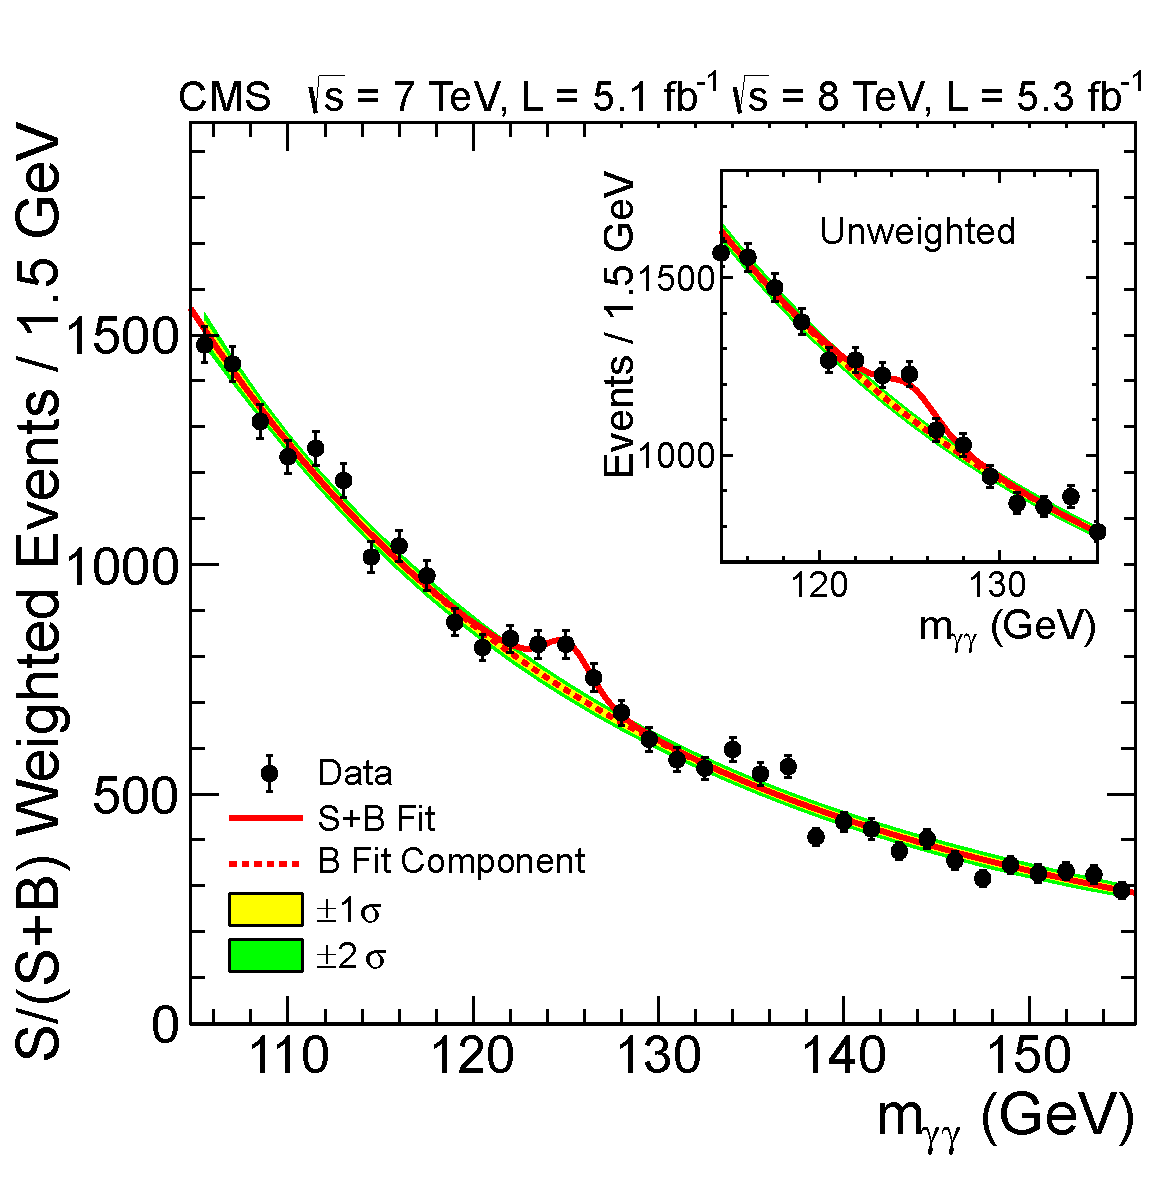
\includegraphics[width=0.49\columnwidth]{figures_chapter2/gammagamma}
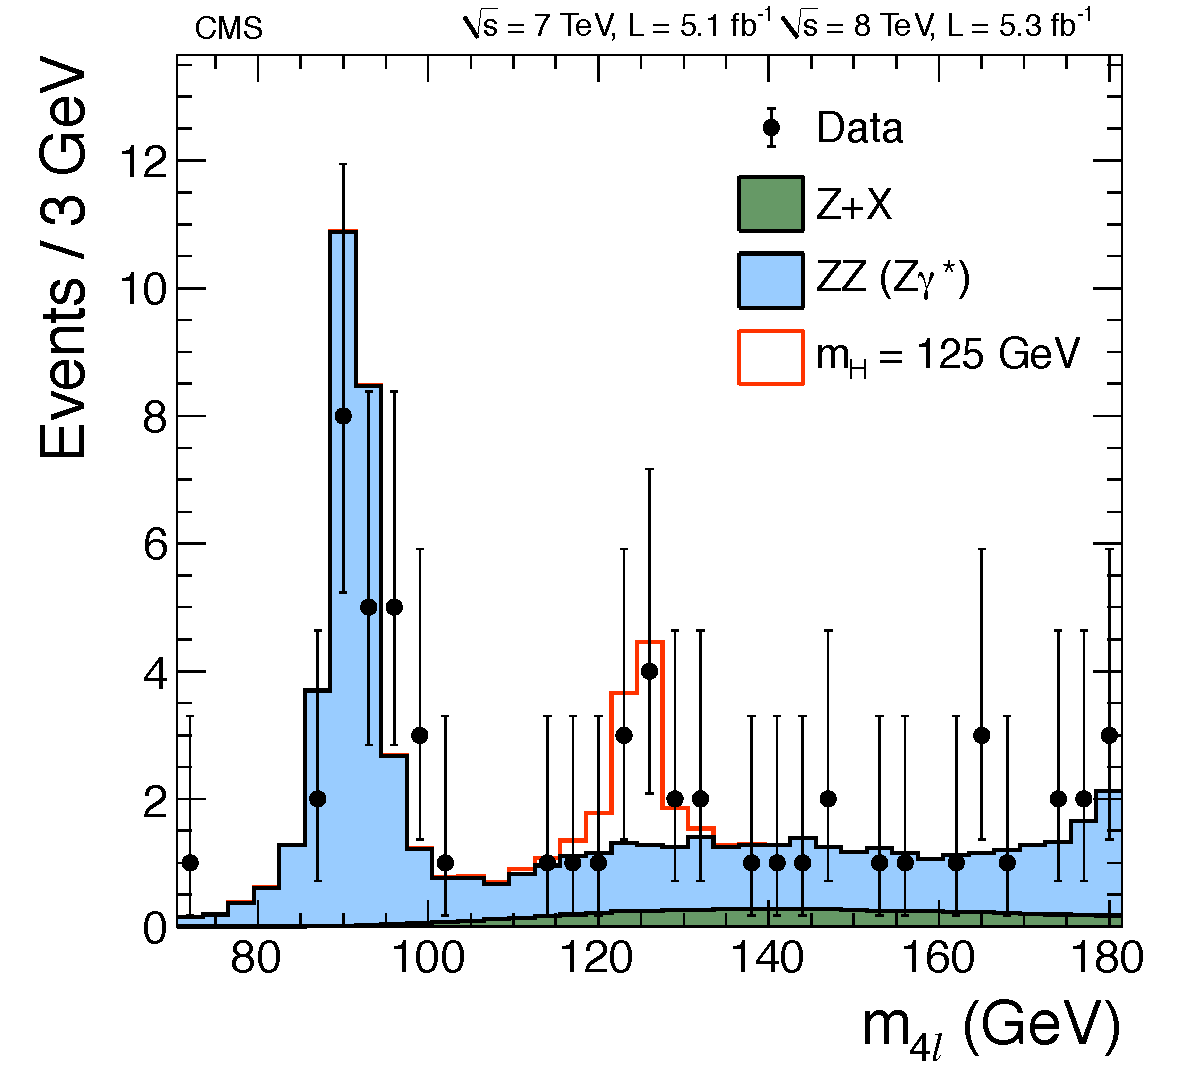
\includegraphics[width=0.49\columnwidth]{figures_chapter2/zz4l}
\caption{Distributions of the diphoton invariant mass with each event weighted by $S/(S+B)$ value (left panel) and the four-lepton invariant mass for the $ZZ \rightarrow 4 \ell$ decays (right panel)~\cite{Chatrchyan:2012xdj}.}
\label{fig:cms_higgs}
\end{figure}

The search for the SM Higgs boson has been one of the highlights of the Large Hadron Collider (LHC)~\cite{1748-0221-3-08-S08001}. In July 2012, the ATLAS and CMS collaborations announced the observation of a narrow resonance with a mass of about $125~\GeV$ with properties consistent with the SM Higgs boson~\cite{Aad:2012tfa,Chatrchyan:2012xdj}. Significant excesses were observed in $\gamma\gamma$ and $ZZ$ decay modes with rates consistent with the SM predictions. There were also strong hints in the data that the new particle decays to $W^+W^-$. The observed decay channels indicate that the new particle is a boson. Figure~\ref{fig:cms_higgs} shows the distributions of the diphoton invariant mass (weighted by the signal-to-background ratio) and four-lepton invariant mass for the $ZZ \rightarrow 4\ell$ decays in the CMS results. The ATLAS and CMS continued to take data after the discovery announcement. Subsequent measurements of the Higgs boson production and decay rates, combining the ATLAS and CMS results, with proton-proton collisions at centre-of-mass energies of $7$ and $8~\TeV$ show a consistent picture with the SM Higgs predictions~\cite{Khachatryan:2016vau}. The combined measured mass of the discovered boson is $m_{H}=125.09 \pm 0.21 \mathrm{(stat.)} \pm 0.11 \mathrm{(syst.)}~\GeV$~\cite{Aad:2015zhl}. The spin and CP properties of the new boson are also consistent with those expected of the SM Higgs boson~\cite{Chatrchyan:2012jja,Aad:2013xqa,Khachatryan:2014kca}.

The measurement of the Higgs boson decays to $b\bar{b}$ and $\tau^{+}\tau^{-}$ is essential for identifying if the new boson is the SM Higgs boson. Both decay modes provide a direct probe of the Higgs Yukawa coupling to fermions. The $\tau^{+}\tau^{-}$ decay mode is currently the most promising channel to study the SM Higgs boson coupling to leptons.

\section{Overview of the Standard Model}

\subsection{Quantum Chromodynamics}

The gauge group of the strong interactions of the colored quarks and gluons is $SU(3)$. The most general gauge invariant and renormalizable Lagrangian of the quantum chromodynamics (QCD) is given by:
 \begin{equation} \label{eq:qcd_lang}
\mathcal{L} =  \bar{\psi}_{f,\alpha} (i \gamma^{\mu}\partial_{\mu}\delta_{\alpha\beta}-g_{s}\gamma^{\mu}t^{a}_{\alpha\beta}A^{a}_{\mu}-m_{f}\delta_{\alpha\beta})\psi_{f,\beta}-\frac{1}{4}F_{\mu\nu}^{b}F^{b,\mu\nu}-\theta\frac{g_{s}^2}{72\pi^2}\epsilon_{\mu\nu\rho\sigma}F^{c,\mu\nu}F^{c,\rho\sigma},
\end{equation}
where repeated indices are summed over. The $\psi_{f,\alpha}$ are the quark-field Dirac spinors of flavor $f$, color $\alpha$, and mass $m_{f}$. There are $6$ quark flavors, the up (u), charm (c), and top (t) each carrying an electric charge of $+2e/3$, and the down (d), strange (s), and bottom (b) each carrying an electric charge of $-e/3$. Each quark flavor comes in three "colors" transforming according to the fundamental representation of the $SU(3)$ color group. The $A_{\mu}^{a}$ denotes the massless gluon field vector potentials transforming according to the adjoint representation of the $SU(3)$ color group with $a$ running from $1$ to $N_{c}^2-1=8$ (8 gluons).  The $t_{\alpha\beta}^{a}$ are the eight generators of the color group represented by $3 \times 3$ Hermitian traceless matrices. The $g_{s}$ (or $\alpha_{s} = \frac{g_{s}}{4\pi}$) is the strong interaction coupling constant, the $\gamma^{\mu}$ are the Dirac matrices, and the gauge field tensor is given by:
 \begin{eqnarray} \label{eq:qcd_field}
 \begin{aligned}
F_{\mu\nu}^{a} &= \partial_{\mu}A_{\nu}^a-\partial_{\nu}A_{\mu}^a-g_{s}f_{abc}A_{\mu}^{b}A_{\nu}^{c},  \\
\mathrm{[}t^a,t^b\mathrm{]} &= if_{abc}t^{c},
\end{aligned}
\end{eqnarray}
where $f_{abc}$ are the structure constants of the $SU(3)$. The non-Abelian structure of the $SU(3)$ group means that the Feynman rules of QCD involve 3-gluon and 4-gluon vertices in addition to the quark-antiquark-gluon vertex. The last term in the Lagrangian in Eq.~(\ref{eq:qcd_lang}) can induce an electric dipole moment for the neutron resulting in a CP violation. However the experimental limits on the electric dipole moment constrain the $\theta$ parameter to be smaller than $10^{-10}$~\cite{Agashe:2014kda}. This is known as the strong CP problem with a possible resolution given by the Peccei-Quinn theory predicting the existence of a hypothetical particle Axion~\cite{PhysRevLett.38.1440}. There are $7$ fundamental parameters in the QCD Lagrangian (not counting the $\theta$ parameter): the $6$ quark masses and the strong coupling $g_{s}$ constant.
Predictions utilizing perturbative QCD (pQCD) calculations are expressed in terms of the renormalized coupling constant $g_{s} (\mu_R)$ as a function of a non-physical renormalization scale $\mu_R$. The renormalization group equation to three-loop order is given by:
\begin{eqnarray} \label{eq:qcd_rge}
\mu\frac{d}{d\mu}g_s{\mu_R} = - (\beta_{0} \frac{g_{s}^{3}(\mu_R)}{16\pi^2} +  \beta_{1} \frac{g_{s}^{5}(\mu_R)}{128\pi^4} + \beta_{2} \frac{g_{s}^{7}(\mu_R)}{8192\pi^6}),
\end{eqnarray}
where the loop coefficients $\beta_{i}$ are:
\begin{eqnarray} \label{eq:qcd_beta}
\begin{aligned}
\beta_{0}&=11-\frac{2}{3}n_{f}, \\
\beta_{1}&=51-\frac{19}{3}n_{f}, \\
\beta_{2}&=2857-\frac{5033}{9}n_{f}-\frac{325}{27}n_{f}^2,
\end{aligned}
\end{eqnarray}
and $n_{f}$ is the number of quark flavors with masses below the energies of interest~\cite{Agashe:2014kda}. The minus sign in Eq.~(\ref{eq:qcd_rge}) is the source of the asymptotic freedom and as can be seen in Eq.~(\ref{eq:qcd_beta}) the theory is asymptotically free as long as there are less than $16$ quark flavors below the energy scale of interest. Setting the renormalization scale near the momentum transfer $Q$ of a given process gives the effective strength of the strong coupling. Thus the strong coupling becomes weak for larger $Q$ and $\alpha_{s} \approx 0.1$ for momentum transfers near $100~\GeV$. Free quarks and gluons have not been observed experimentally. The asymptotic freedom implies that the strong coupling increases at low energies (large distances) and only color-singlet combinations of quarks, massless gluons, and anti-quarks, referred as hadrons, can be observed.  
 
\subsection{Electroweak Model}

The gauge group of the electroweak interactions is $SU(2) \times U(1)$ with the corresponding gauge bosons $\vec{W}_{\mu}$ and $B_{\mu}$ respectively. The $SU(2)$ part of the gauge group is chiral, i.e. it only acts on the left-handed components of the quark and lepton fields. The left handed fermion fields transform as doublets under $SU(2)$ and are given by:
\begin{eqnarray} \label{eq:doublet}
\Psi  = \left(\begin{array}{c} \nu_{f}\\ \ell_{f} \end{array} \right)\mathrm{,}  \quad \left(\begin{array}{c} \nu_{\mu}\\ \mu \end{array} \right)\mathrm{,}   \quad \left(\begin{array}{c} \nu_{\tau}\\ \tau \end{array} \right),
\end{eqnarray}   
for each lepton generation and by:
\begin{eqnarray} \label{eq:doublet_quark}
\Psi  = \left(\begin{array}{c} u \\ d^{'} \end{array} \right)\mathrm{,}  \quad \left(\begin{array}{c} c\\ s^{'} \end{array} \right)\mathrm{,}   \quad \left(\begin{array}{c} t\\ b^{'} \end{array} \right),
\end{eqnarray}   
for the three quark flavors. The $d^{'}$, $s^{'}$, and $b^{'}$ are given by:
\begin{eqnarray} \label{eq:ckm}
\begin{aligned}
d^{'} &= V_{ud}d + V_{us}s + V_{ub}b, \\
s^{'} &= V_{cd}d + V_{cs}s + V_{cb}b, \\
b^{'} &= V_{td}d + V_{ts}s + V_{tb}b, 
\end{aligned}
\end{eqnarray}   
where $V$ is the unitary Cabibbo-Kobayashi-Maskawa (CKM) mixing matrix~\cite{Cabibbo:1963yz,Kobayashi:1973fv}. The right handed fermion fields are $SU(2)$ singlets. The most general gauge invariant and renormalizable Lagrangian for the fermion fields $\psi_{i}$ is given by:
\begin{equation} \label{eq:ewk_ym}
\mathcal{L} = \sum_{i} \bar{\psi}_{i} \gamma^{\mu}(i \partial_{\mu}-\frac{g^{'}}{2}YB_{\mu}) \psi_{i}  - \bar{\Psi}_{i}\gamma^{\mu}\frac{g}{2}\vec{\sigma}\cdot\vec{W}_{\mu}\Psi_{i} - \frac{1}{4}\vec{W}_{\mu\nu}\cdot\vec{W}^{\mu\nu} - \frac{1}{4} B_{\mu\nu} B^{\mu\nu},
\end{equation}
where $g^{'}$ and $g$ are the gauge coupling constants of the $U(1)$ and $SU(2)$ respectively. Thus the $\frac{Y}{2}$, where $Y$ is the weak hypercharge, and the $\frac{1}{2}\vec{\sigma}$, where $\sigma_{i}$ are the Pauli matrices, are the generators of the $U(1)$ and $SU(2)$ respectively. The gauge field tensors are given by:
\begin{eqnarray} \label{eq:ewk_field}
\begin{aligned}
B_{\mu\nu} &= \partial_{\mu}B_{\nu}-\partial_{\nu}B_{\mu}  \\
\vec{W}_{\mu\nu} &=  \partial_{\mu}\vec{W}_{\nu}-\partial_{\nu}\vec{W}_{\mu} + g \vec{W}^{\mu} \times \vec{W}^{\nu}.
\end{aligned}
\end{eqnarray}
The hypercharge is normalized such that the electric charge $Q=\frac{1}{2}\sigma^3+\frac{Y}{2}$. The vector fields corresponding to particles with spin $1$ and definite mass are the charged $W^{\pm}_{\mu}$ bosons, the neutral $Z_{\mu}$ boson and the photon $A_{\mu}$ given in terms of the gauge fields as: 
\begin{eqnarray} \label{eq:bosons}
\begin{aligned}
A_{\mu} &= B_{\mu} \cos \theta + W_{\mu}^{3} \sin \theta \\
Z_{\mu} &= -B_{\mu} \sin \theta + W_{\mu}^{3} \sin \theta \\
W_{\mu}^{\pm} &= W^{1}_{\mu} \mp i W_{\mu}^{2},
\end{aligned}
\end{eqnarray}
where $\theta$ is the weak angle related to the gauge coupling constants by:
\begin{eqnarray} \label{eq:coupling}
\begin{aligned}
\sin \theta &= \frac{g^{'}}{\sqrt{g^2+g^{'2}}} \\
\cos \theta &= \frac{g}{\sqrt{g^2+g^{'2}}}.
\end{aligned}
\end{eqnarray}
However this theory of the electroweak interactions given in Eq.~(\ref{eq:ewk_ym}) is not satisfactory. It contains four massless bosons whereas only the photon is massless in nature. Attempting to add mass terms of the form $-M_{Z}^2Z_{\mu}Z^{\mu}$ for the vector boson fields in the Lagrangian breaks the gauge invariance. Furthermore introducing explicit mass terms for the spin-1 boson fields makes the theory non-renormalizable. There are also no mass terms in the Lagrangian for the fermion fields.  The Dirac fermion mass terms link the left and right-handed components of the fields:
\begin{eqnarray} \label{eq:fermion}
m\bar{\psi}\psi = m(\bar{\psi}_L\psi_R+\bar{\psi}_R\psi_L).
\end{eqnarray}
This breaks the symmetry as the left and right-handed components transform differently under the $SU(2)$ and $U(1)$. Spontaneous symmetry breaking mechanism leaving the underlying gauge symmetry intact was the solution to the conundrum on how the gauge bosons can acquire mass. 

\subsection{The SM Higgs mechanism}

Spontaneous symmetry breaking occurs when the ground state (vacuum) does not exhibit the symmetry of the theory. A key aspect is that the vacuum is degenerate and it can not be predicted in advance which state will be chosen. Taking a precedence from the superconductivity phenomenon it was reasoned that the gauge symmetry can be broken through spontaneous symmetry breaking~\cite{Nambu:1960tm,Anderson:1963pc}. The main difficulty is the appearance of the massless spin-$0$ Nambu-Goldstone bosons after the spontaneous symmetry breaking (the Goldstone theorem~\cite{Goldstone:1962es}) as no such particles are observed. Englert, Brout, Higgs, Guralnik, Hagen, and Kibble showed that the theorem does not apply to the gauge theories ~\cite{Englert:1964et,Higgs:1964ia,Higgs:1964pj,Guralnik:1964eu,Higgs:1966ev,Kibble:1967sv}.  Taking these ideas Weinberg and Salam completed the electroweak unification started by Glashow~\cite{Glashow:1961tr,Weinberg:1967tq,Salam:1968rm}. They also added the possibility to generate the fermion masses through the same spontaneous symmetry breaking. Finally it was proved by t'Hooft and Veltman that this model is renormalizable~\cite{tHooft:1972fi}. 

The $SU(2)$ symmetry is broken by introducing a scalar field (Higgs) in the spinor representation of the $SU(2)$ 
\begin{eqnarray} \label{eq:lang_higgs}
\Phi  = \frac{1}{\sqrt{2}}\left(\begin{array}{c} \sqrt{2}\phi^{+}\\ \phi_{0}+ia^{0} \end{array} \right),
\end{eqnarray}   
with four real degrees of freedom in the complex doublet and weak hypercharge of $Y=1$. The most general renormalizable Lagrangian of the scalar field consistent with $SU(2) \times U(1)$ is given by
\begin{equation} \label{eq:ewk_higgs}
\mathcal{L}_{\Phi} = (D_{\mu}\Phi)^{\dagger} (D^{\mu}\Phi) - \mu^2 \Phi^{\dagger}\Phi - \lambda (\Phi^{\dagger}\Phi)^2,
\end{equation}
with $\lambda>0$. The covariant derivative, given by
\begin{equation} \label{eq:higgs_cov}
D_{\mu}\Phi = (\partial_{\mu}+\frac{1}{2}ig\vec{\sigma}\cdot\vec{W}_{\mu}+\frac{1}{2}g^{'}iYB_{\mu})\Phi,
\end{equation}
is responsible for the Higgs field couplings to the $\vec{W}_{\mu}$ and $B_{\mu}$ gauge fields. There is a tree-approximation non-zero vacuum expectation value (VEV) for $\mu^2<0$ given by:
\begin{eqnarray} \label{eq:vev}
<\Phi>  =  \left(\begin{array}{c} 0\\ \frac{1}{\sqrt{2}}\nu \end{array} \right),
\end{eqnarray}    
with VEV $\nu^2= -\frac{\mu^2}{\lambda}$. A $SU(2)\times U(1)$ gauge transformation was performed in Eq.~(\ref{eq:vev}) to a unitary gauge in which $\phi^{+}=0$, and $a^{0}=0$ leaving a positive $<\phi^{0}>$. Defining $\phi^{0}=H+\nu$ in the Lagrangian in Eq.~(\ref{eq:ewk_ym}) induces the spontaneous breaking of the SM gauge symmetry $SU(2)\times U(1)$ into $U(1)_{em}$ group. The generator of the $U(1)_{em}$ gauge group is the electric charge $Q=\frac{1}{2}\sigma^3+\frac{Y}{2}$. Thus the photon field $A_{\mu}$ remains massless and the Higgs Lagrangian is given by
 \begin{eqnarray} \label{eq:ewk_higgs2}
 \begin{aligned}
\mathcal{L_{H}} &= \frac{1}{2} \partial_{\mu}H\partial^{\mu}H - \frac{1}{2} m_{H}^2 H^2 -\frac{1}{2}m_{W}^2W_{\mu}^{+}W^{-\mu} - \frac{1}{2}m_{Z}^2Z_{\mu}Z^{\mu}  \\
&+ \frac{m_{H}^2}{2\nu} H^3 + \frac{m_{H}^2}{8\nu^2} H^4 + \frac{m_{Z}^2}{\nu} Z_{\mu}Z^{\mu}H + \frac{2m_{W}^2}{\nu} W^{+}_{\mu}W^{-\mu} H  \\
&+ \frac{m_{Z}^2}{2\nu^2} Z_{\mu}Z^{\mu} H^2 +\frac{m_{W}^2}{\nu^2} W^{+}_{\mu}W^{-\mu} H^2,
\end{aligned}
\end{eqnarray}
where the Lagrangian is expressed in terms of the $W_{\mu}^{\pm}$ and $Z_\mu$ fields given in Eq.~(\ref{eq:bosons}) and
 \begin{eqnarray} \label{eq:masses}
 \begin{aligned}
m_{H}  &= \sqrt{-2\mu^2} \\
m_{W} &= \frac{1}{2}g\nu = \cos\theta m_{Z} \\
m_{Z} &= \frac{1}{2} \sqrt{g^2+g^{'2}}\nu \\
m_{A} &= 0.
\end{aligned}
\end{eqnarray}
Thus the spin-$1$ gauge bosons $W_{\mu}^{\pm}$ and $Z_\mu$ have acquired mass. The Higgs boson field H is also massive. The three scalar fields in Eq.~(\ref{eq:lang_higgs}) are "eaten" by the $W_{\mu}^{\pm}$ and $Z_\mu$ fields and the fourth remains as the neutral Higgs field. One can see that the Higgs boson couplings to the spin-$1$ vector bosons are proportional to the mass squared of the bosons. The Higgs boson trilinear and quartic self couplings are proportional to the $m_{H}^2$.

The final item needed to complete the theory is to add a mechanism for generating the fermion masses. The fermions acquire mass through a Yukawa type interactions between the Higgs scalar field and the fermions. The Yukawa Lagrangian before the electroweak symmetry is given by:
\begin{eqnarray} \label{eq:yukawa}
\mathcal{L_{\mathrm{Y}}} = -h_{d_{ij}} \bar{q}_{L_{i}} \Phi d_{R_j}  - h_{u_{ij}} \bar{q}_{L_{i}} i\sigma^{2}\Phi^{*}d_{R_j} - h_{\ell_{ij}} \bar{\ell}_L \Phi e_{R_j} + \quad \mathrm{h.c.}, 
\end{eqnarray}   
where the $q_L$ ($\ell_L$) and $u_R$, $d_R$ ($e_R$) are the quark (lepton) $SU(2)$ doublets (singlets) and the $3\times3$ matrices are the couplings~\cite{Agashe:2014kda}. After the electroweak symmetry breaking and rotating to the fermion mass eigenstate basis the coupling matrices are diagonalized and the fermions acquire masses given by $m_{f} = \frac{h_f \nu}{\sqrt{2}}$. The Higgs to fermion coupling term becomes $\frac{m_{f}}{\nu}\bar{f}fH$. Thus the fermions have acquired mass and the Higgs coupling to the fermions is proportional to the mass of the fermion in question. The Dirac neutrino masses can also be included in this framework if one considers the right handed neutrinos. It has to be noted that the fermion mass parameters have been replaced by the Yukawa couplings. Finally the Lagrangian for the fermion fields $\psi_{i}$ after the electroweak symmetry breaking reads:
\begin{eqnarray} \label{eq:lf}
\begin{aligned}
\mathcal{L_F} &= \sum_{i} \bar{\psi}_{i} (i\partial - m_{i} - \frac{m_{i}H}{\nu}) \psi_{i} -\frac{g}{2\sqrt{2}}\sum_{i}\bar{\Psi}_i \gamma^{\mu}(1-\gamma^5)(T^{+}W_{\mu}^{+} + T^{-} W_{\mu}^{-})\Psi_{i}  \\
& -e\sum_{i} Q_i \bar{\psi}_{i} \gamma^{\mu} \psi_i A_{\mu} - \frac{g}{2\cos\theta}\sum_{i}\bar{\psi}_i \gamma^{\mu}(g_{V}^{i}-g_{A}^{i}\gamma^{5})\psi_{i}Z_{\mu}, 
\end{aligned}
\end{eqnarray}
where $e=g \sin \theta$ is the magnitude of the electron electric charge. The vector and axial-vector couplings are given as $g_{A}^{i}=t^{i}_{3}$ and $g_{V}^{i}=t^{i}_{3}-2Q^{i} \sin^{2} \theta$, where the  $t^{i}_{3}$ is the weak isospin of fermion $i$. The $T^{\pm}$ are the weak isospin raising and lowering operators. The source of the CP violation in the Lagrangian is encoded in the CKM matrix.

It is interesting to consider the number of free parameters in the SM (ignoring the the neutrino masses). There are $9$ Yukawa couplings for each fermion. The CKM matrix is unitary and thus has $4$ parameters. The $3$ coupling constants for each gauge component: $g_s$, $g$, $g^{'}$, the vacuum expectation value ($\nu$), the self coupling parameter $\lambda$ of the Higgs field, and the $\theta$ in the QCD Lagrangian are the remaining parameters. Thus, there are $19$ free parameters in the SM theory of elementary particles. 

\subsection{Extended Higgs Sector}

The SM theory of elementary particles has been remarkably successful in describing the present experimental observations. However there are number of undesirable aspects of the theory necessitating an effort to improve our understand of nature. The large number of free parameters in the model ($19$), the strong CP problem, the naturalness problem, the inclusion of gravity in the SM, and understanding the generation of the neutrino masses are few examples to consider. There is also no candidate for the non-baryonic dark matter in the SM. 

The SM Higgs boson is a scalar particle and is therefore susceptible to the ultraviolet (UV) divergent radiative quadratic loop corrections. For example, a Dirac fermion loop introduces a correction to the Higgs boson mass given by:
\begin{eqnarray} \label{eq:hierarchy}
m^{2}_{SM} = m^2_{\mathrm{bare}} - \frac{|\lambda_f|^2}{16\pi^2} \Lambda^2, 
\end{eqnarray}
where the $\lambda_f$ is the Yukawa coupling and $\Lambda$ is the ultraviolet cut-off scale. If the cut-off scale is at the Planck scale of $10^{19}~\GeV$  then dramatic cancellations (fine tuning) are required on the right hand side of the Eq.~(\ref{eq:hierarchy}) to achieve a Higgs mass of the order of the electroweak scale. Supersymmetry is one of the proposed solutions to this naturalness problem where one introduces a new symmetry in nature between the bosons and fermions~\cite{Golfand:1971iw,Wess:1974tw}. A detailed introduction to the supersymmetry can be found in~\cite{Martin:1997ns}. The quadratic corrections to the Higgs mass have opposite signs for the fermion and boson loop corrections. In supersymmetry theories every SM fermion (boson) has a super-partner boson (fermion) providing a natural cancelation of the quadratic loop divergences. The supersymmetry is a broken symmetry as there are no hints of the super-partners in the experimental data. The naturalness problem is still a concern if the scale at which the symmetry breaks is larger than $1~\TeV$.  

The Minimal Supersymmetric Standard Model (MSSM) is the simplest extension of the SM to include the ideas of the supersymmetry~\cite{Fayet:1974pd,Fayet:1977yc}. The Higgs sector in the MSSM considers an additional scalar Higgs doublet (2HDM) with hypercharge of $Y=-1$ given by:
\begin{eqnarray} \label{eq:2hdm}
\Phi_1  = \frac{1}{\sqrt{2}}\left(\begin{array}{c} \phi^{0}_1+ia_1^0 \\ \sqrt{2}\phi^{-}_1 \end{array} \right), \quad \Phi_2  = \frac{1}{\sqrt{2}}\left(\begin{array}{c} \sqrt{2}\phi^{+}_2 \\ \phi^{0}_2+ia_2^0 \end{array} \right).
\end{eqnarray}    
Analogous to the SM case, the scalar fields acquire vacuum expectation values as the electroweak symmetry is spontaneously broken. There are eight degrees of freedom in the two doublets leading to five physical Higgs particles after the electroweak symmetry breaking:
\begin{eqnarray} \label{eq:mssm_higgs}
\begin{aligned}
H^{\pm} &= \sin \beta \phi_1^{\pm} + \cos \beta \phi_2^{\pm} \\
A  &= \sin \beta \mathrm{Im}\phi_1^{0} + \cos \beta \mathrm{Im}\phi_2^{0} \\
H  &= \cos \alpha(\mathrm{Re}\phi_1^{0}-\nu_1) + \sin \alpha (\mathrm{Re}\phi_2^{0}-\nu_2) \\
h  &= -\sin \alpha(\mathrm{Re}\phi_1^{0}-\nu_1) + \cos \alpha (\mathrm{Re}\phi_2^{0}-\nu_2),
\end{aligned}
\end{eqnarray}   
where $\nu_i=<\phi_i^0>$ are the vacuum expectation values satisfying the requirement $\nu_{SM}^2 = \nu_1^2 + \nu_2^2$. Thus, there are two neutral CP-even states $h$ and $H$, and one neutral CP-odd state $A$. There is also a charged Higgs pair $H^{\pm}$. The mixing angle is related to the ratio of the vacuum expectation values: $\tan \beta = \frac{\nu_2}{\nu_1}$. The $h$ ($H$) denotes the light (heavy) CP-even Higgs. The couplings of the $H$ and $A$ bosons to the down type quarks and leptons have an additional factor of $\tan \beta$ enhancing the decay of the heavy neutral bosons to down type fermions for large $\tan \beta$.

At tree level the MSSM Higgs sector is determined by two parameters: $\tan \beta$ and the mass of one of the Higgs bosons ($m_{A}$ is typically chosen). The mass spectrum is given by:
\begin{eqnarray} \label{eq:mssm_mass}
\begin{aligned}
m_{H,h}^2 &= \frac{1}{2} (m_A^2 + m_Z^2 \pm \sqrt{(m_A^2+m_Z^2)^2-4m_Z^2m_A^2\cos^22\beta}), \\
m_{H^{\pm}}^2 &= m_{A}^2 + m_{W}^2.
\end{aligned}
\end{eqnarray}   
For $m_{A}$ much larger than the mass of the $Z$ boson (decoupling limit) the heavy scalars are almost degenerate $m_{H} \approx m_{H^{\pm}} \approx m_{A}$. There is also an upper bound on the lightest Higgs boson given by $m_{h} \leq m_{Z} \cos 2\beta$. However the radiative corrections are important and an upper bound of about $135~\GeV$ is possible~\cite{Degrassi:2002fi}. The strategy in interpreting the experimental results in the MSSM is to fix the parameters that enter through the radiative corrections (benchmark scenarios) and explore the parameter space in $m_{A}-\tan \beta$ plane. The discovery of the Higgs boson at mass of $125~\GeV$ invites to interpret the $h$ as the discovered boson and search for the heavier scalars appearing in the MSSM. Few benchmark scenarios are considered in the results~\cite{Heinemeyer:2011aa,Carena:2013ytb}.

\section{The Large Hadron Collider}
The LHC~\cite{1748-0221-3-08-S08001} is a circular proton-proton collider located at the European Organization for Nuclear Research (CERN). The tunnel has a circumference of $26.7$ km and previously hosted the Large Electron-Positron (LEP)~\cite{lep1,lep2} collider. Located at the border of France and Switzerland, the tunnel lies between $45$ m and $170$ m below the surface. The LHC is designed to collide beams of protons at centre-of-mass energy $\sqrt{s}$ of up to $14~\TeV$. While the LHC is primarily a proton-proton collider, lead (Pb) ion beams of energy of $2.3~\TeV$ per nucleon are used to produce lead-lead  and proton-lead collisions.  
 
Figure~\ref{fig:cern} shows a schematic representation of the accelerator complex at CERN. Ionized hydrogen atoms are accelerated to an energy of $50~\MeV$ in the Linac $2$ linear accelerator. Thereafter they are injected into the Proton Synchrotron Booster (PSB) and Super Proton Synchrotron (SPS) raising the energy to $25~\GeV$ and $450~\GeV$ respectively. From the SPS the protons are injected into two separate rings in discrete bunches. At the design bunch spacing of $25$ ns there are $2808$ proton bunches per beam. 

\begin{figure}[h]
\centering
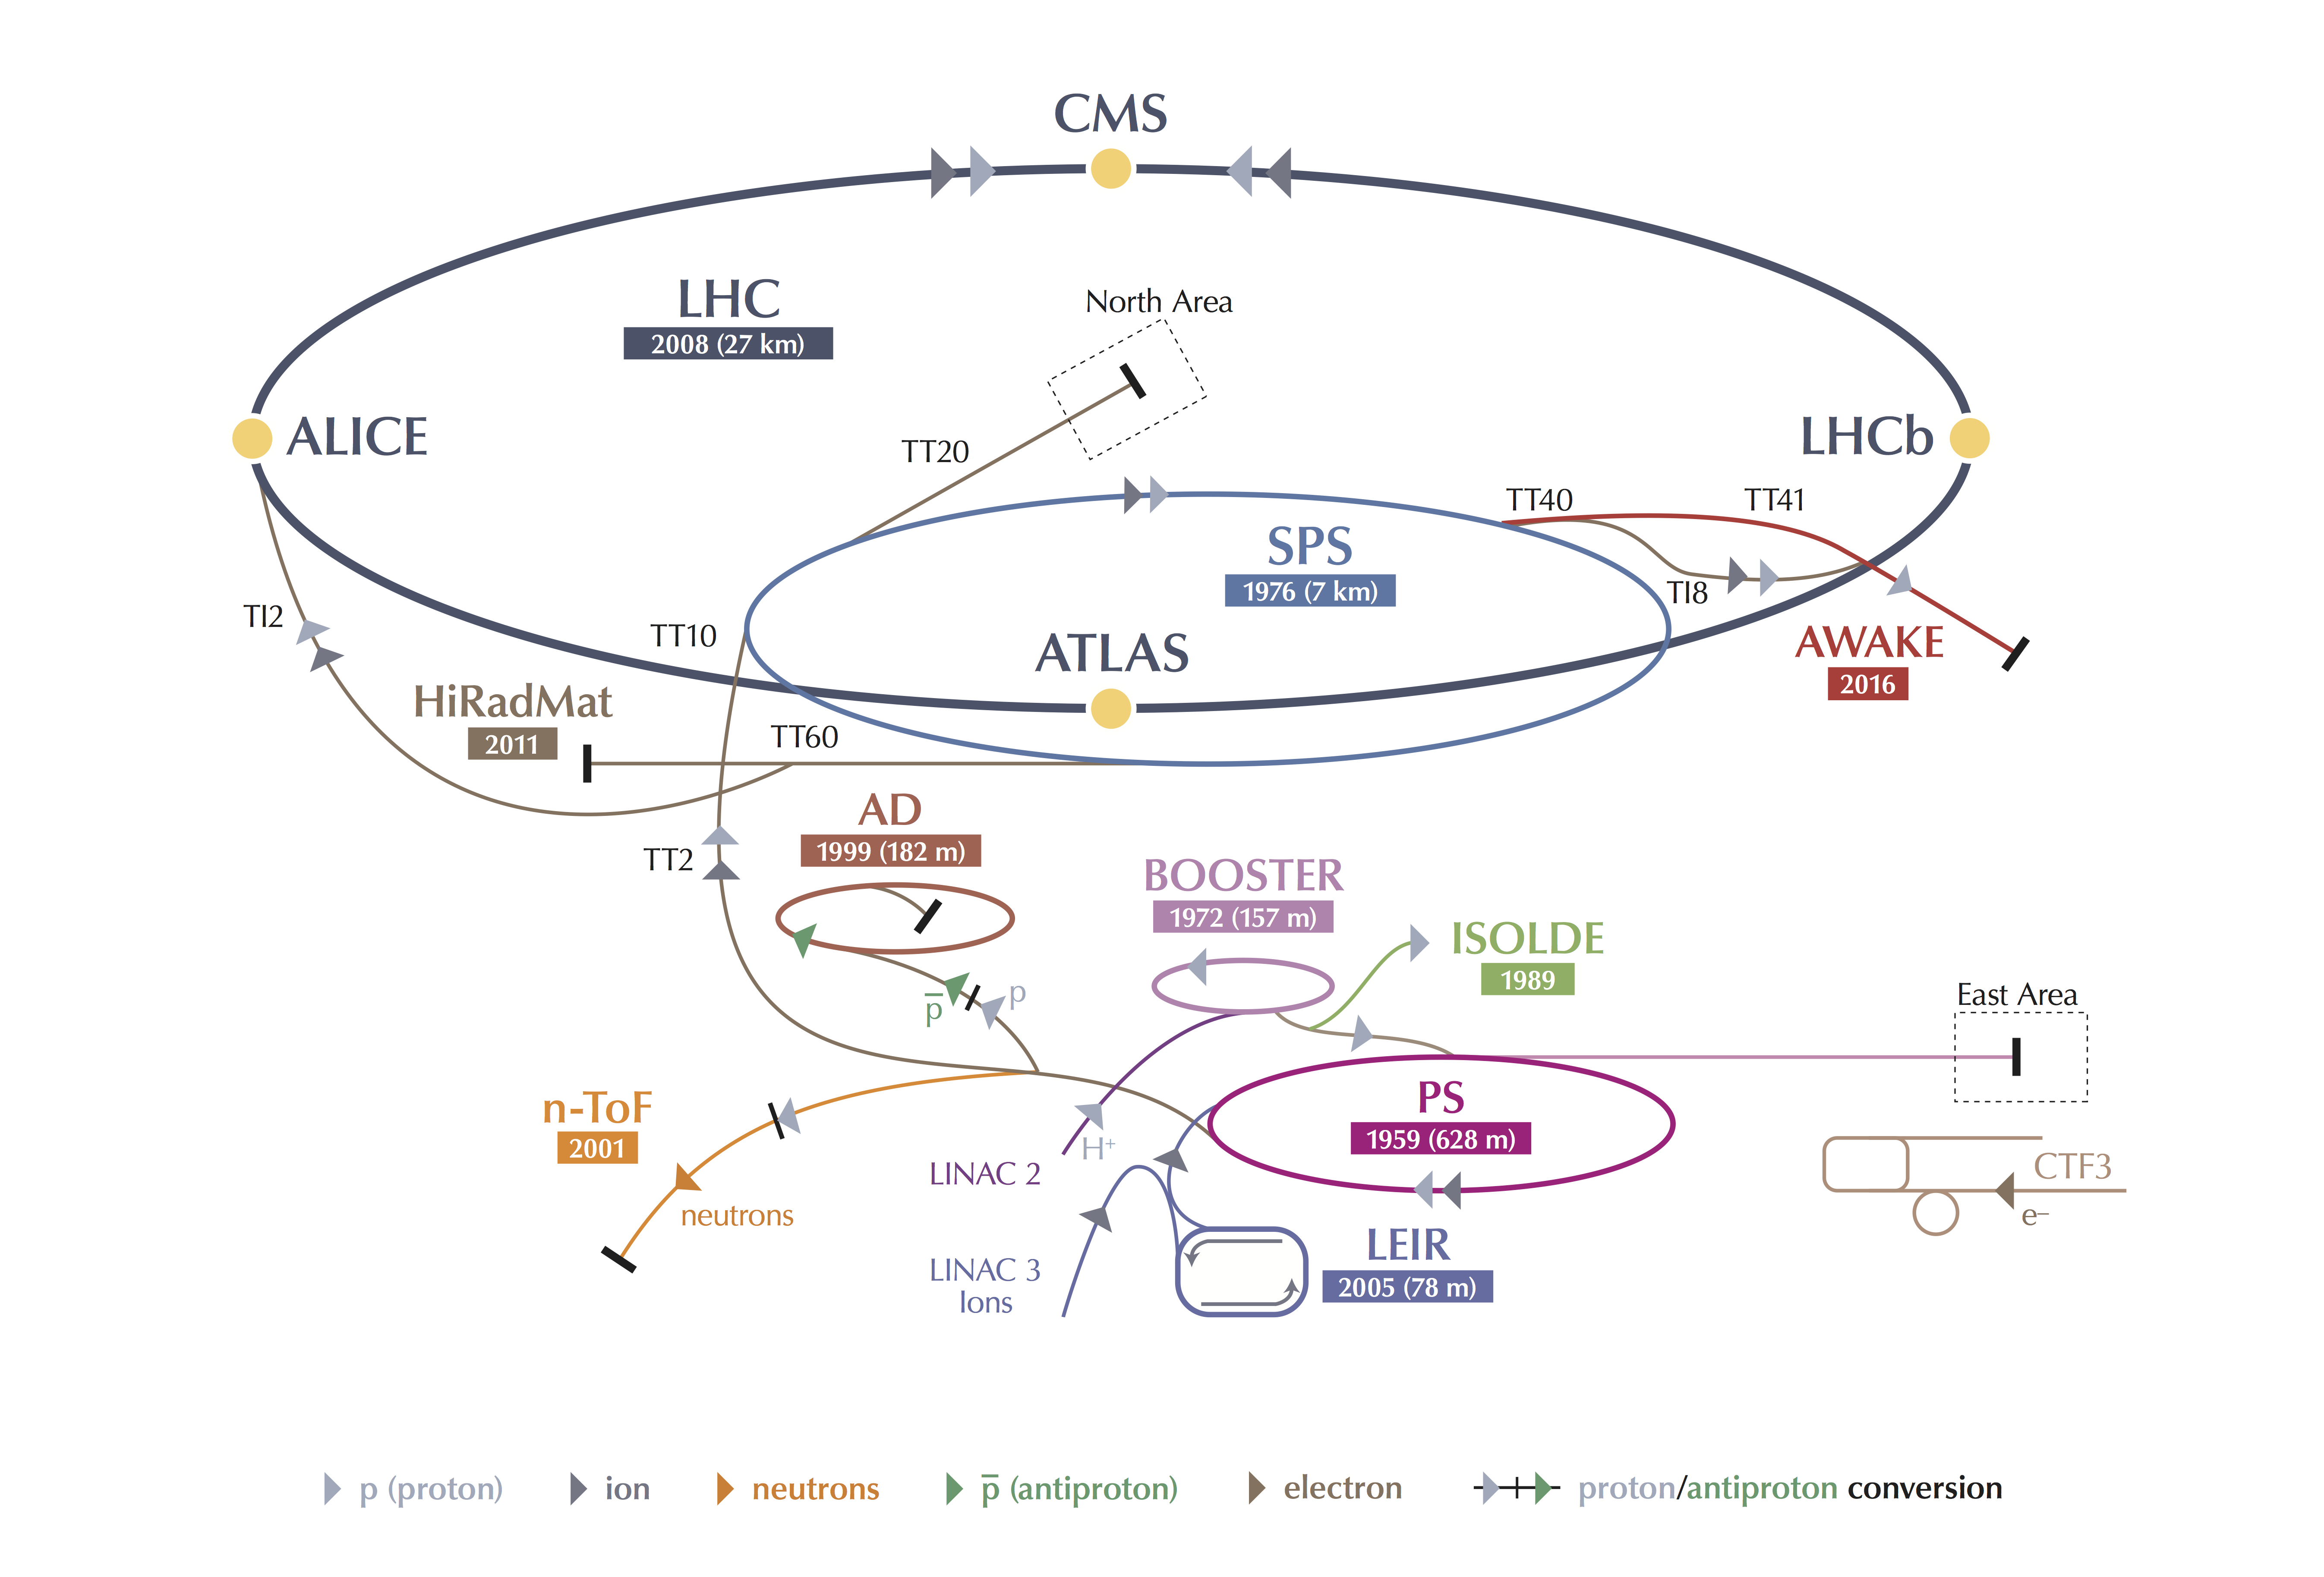
\includegraphics[width=1.0\columnwidth]{figures_chapter2/cern_complex.jpg}
\caption{A schematic representation of the CERN accelerator complex~\cite{Haffner:1621894}.}
\label{fig:cern}
\end{figure}

Using the synchrotron method the design beam energy is achieved with $1232$ dipole magnets (15 meters in length) with a peak dipole field of $8.33$ Tesla. Quadrupole magnets (492) of $5-7$ meters in length are used to focus the beams. Two beam pipes with counter rotating beams are required as the LHC is a particle-particle accelerator.  Space limitations in the tunnels led to the adoption of the twin-bore~\cite{Blewett:1971zzb} magnet design where the beam pipes are magnetically coupled and the magnets share the same mechanical structure and cryostat. The target magnetic field is achieved using niobium-titanium superconducting electromagnets with operating temperatures of $1.9$ K. Superfluid helium is used to cool the magnets to the operating temperature.
   
\begin{figure}[h]
\centering
%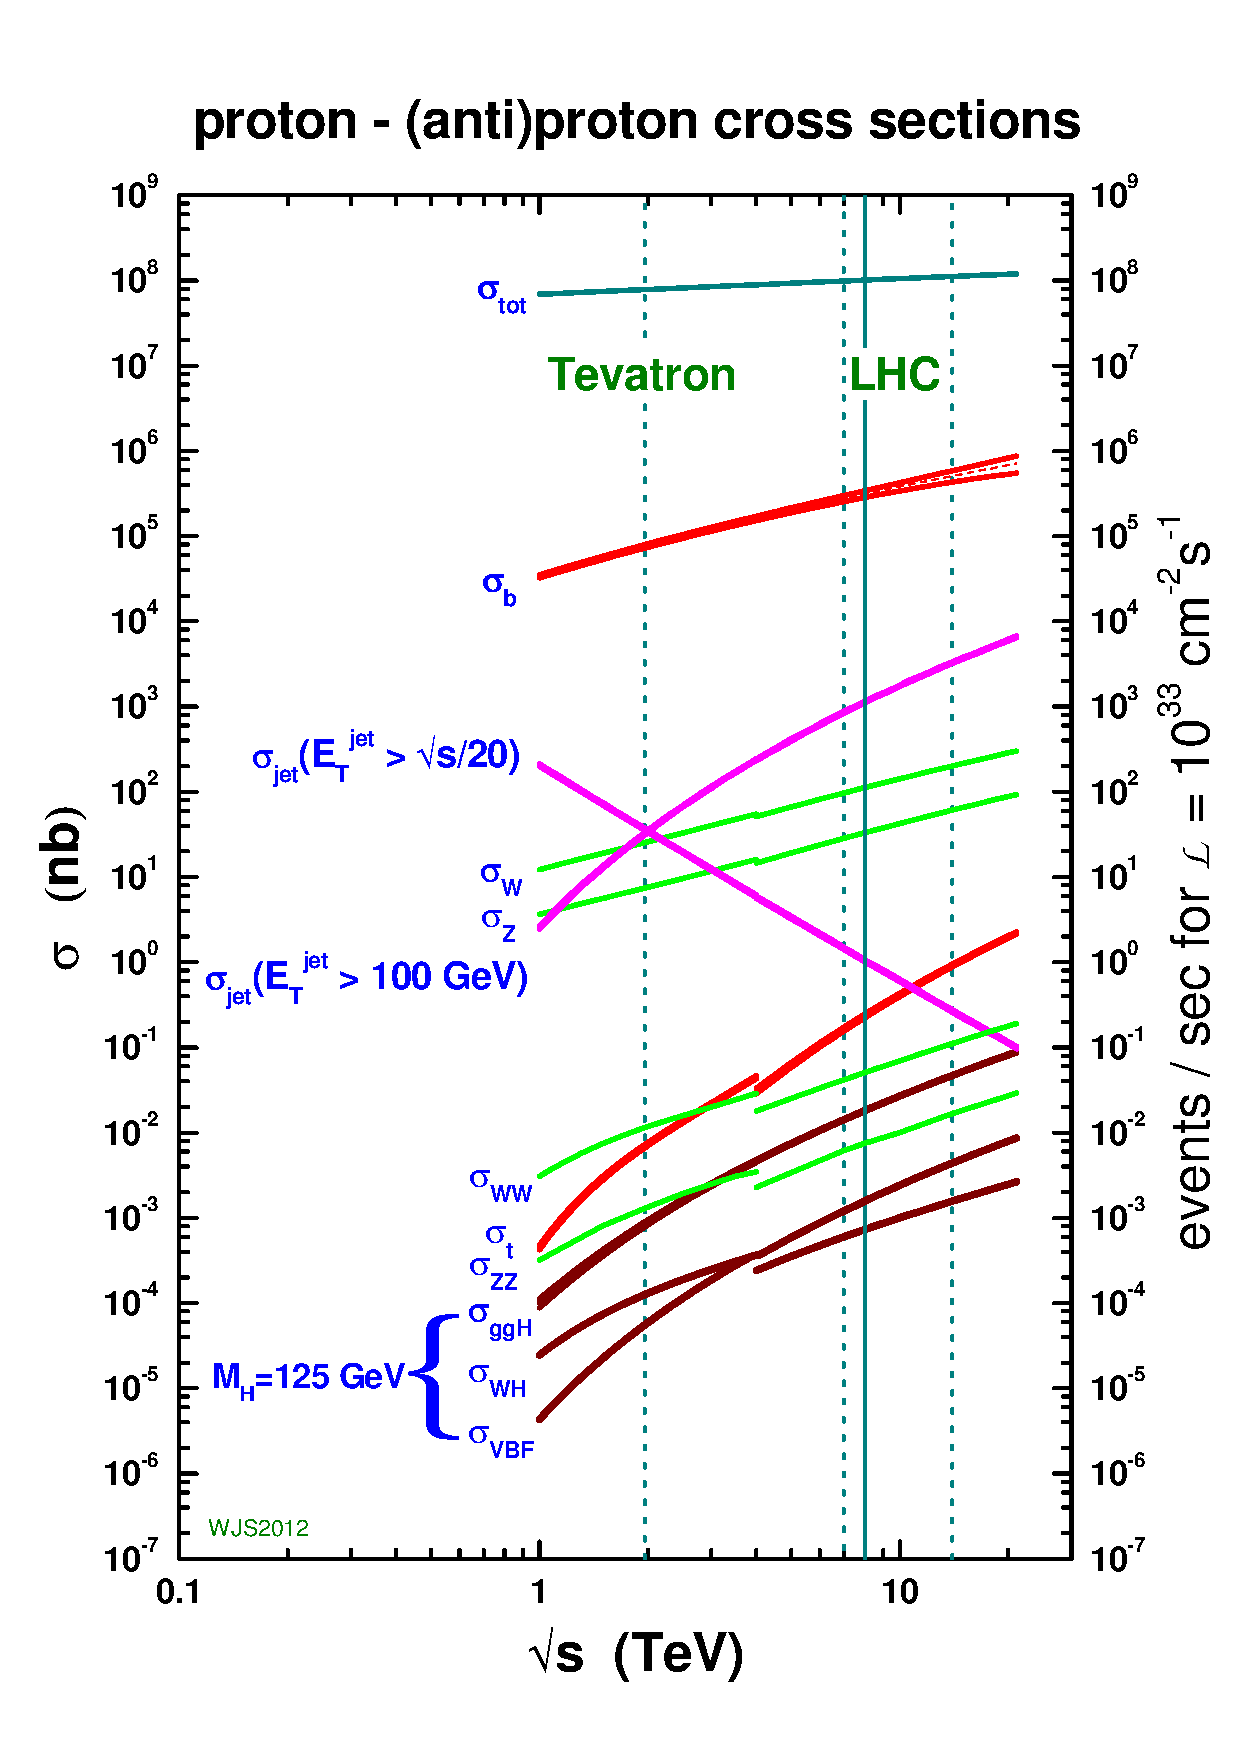
\includegraphics[width=1.0\columnwidth]{figures_chapter2/crosssections2013}
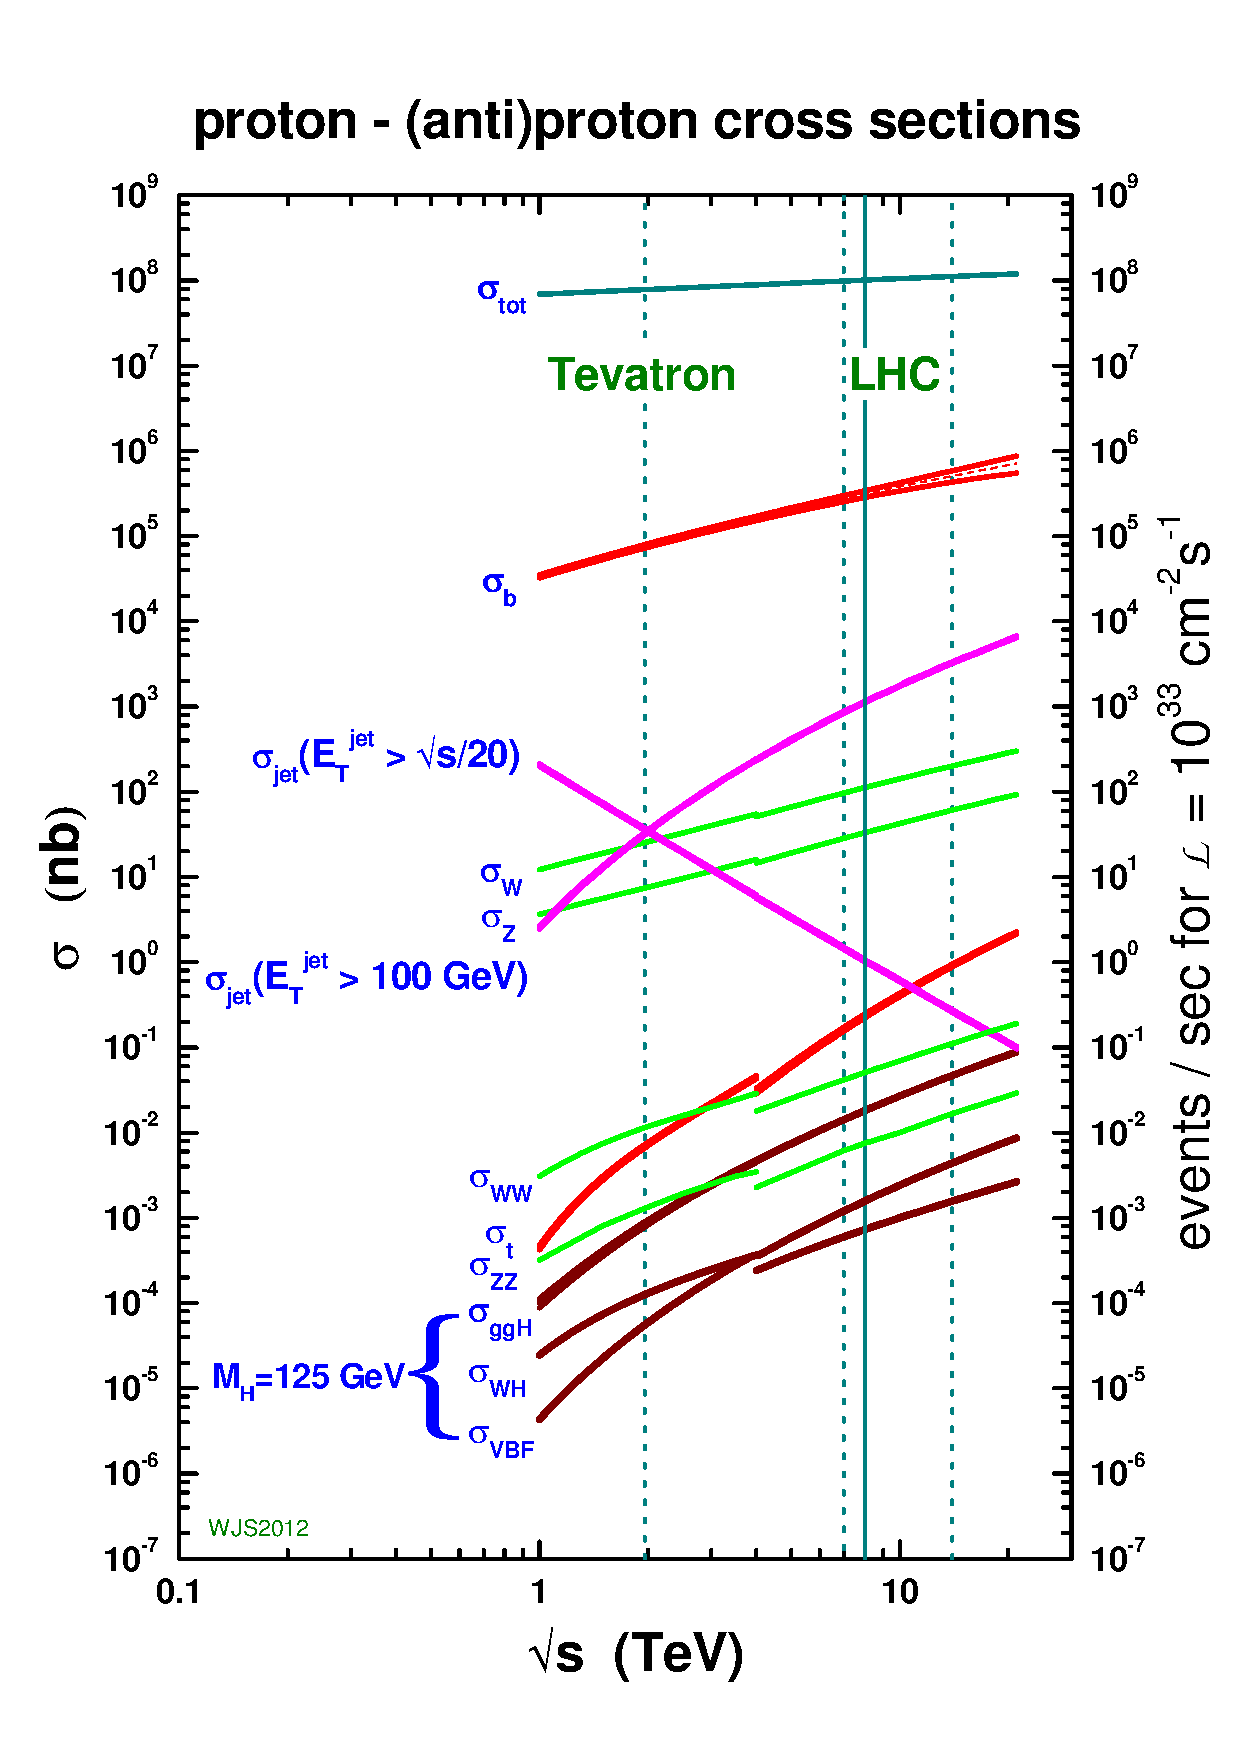
\includegraphics[width=0.5\columnwidth]{figures_chapter2/crosssections2013}
\caption{Cross sections of various SM processes as a function of $\sqrt{s}$ in proton-proton and proton-antiproton collisions~\cite{sterling}. The total hadronic cross section is based on a parameterization from Particle Data Group~\cite{Agashe:2014kda}. The remaining cross sections are calculated at NLO or NNLO using MSTW2008 parton distributions~\cite{MSTW}. The discontinuities illustrate the differences in cross sections between the proton-proton and proton-antiproton collisions.}
\label{fig:xsec}
\end{figure}

The goal of the LHC is to elucidate the mechanism of the electroweak symmetry breaking and to look for hints of beyond the Standard Model (BSM) physics. The rate of events generated in the LHC collisions is given by 
\begin{equation} \label{eq:lumi}
N = \sigma L,
\end{equation}
where $\sigma$ is the cross section of the event under study and $L$ is the luminosity. Figure~\ref{fig:xsec} shows the production cross sections of various SM processes as a function of $\sqrt{s}$ in proton-proton and proton-antiproton collisions. The rear processes of interest at the LHC are orders of magnitude smaller than the total hadronic cross section. Therefore, in addition to high beam energies, high beam intensities are required. The design peak luminosity at the LHC is $10^{34}$ cm$^2$s$^{-1}$ for the proton-proton collisions. The high beam intensity requirement excludes the feasibility of using proton-antiproton collisions at the LHC. 

\begin{figure}[h]
\centering
%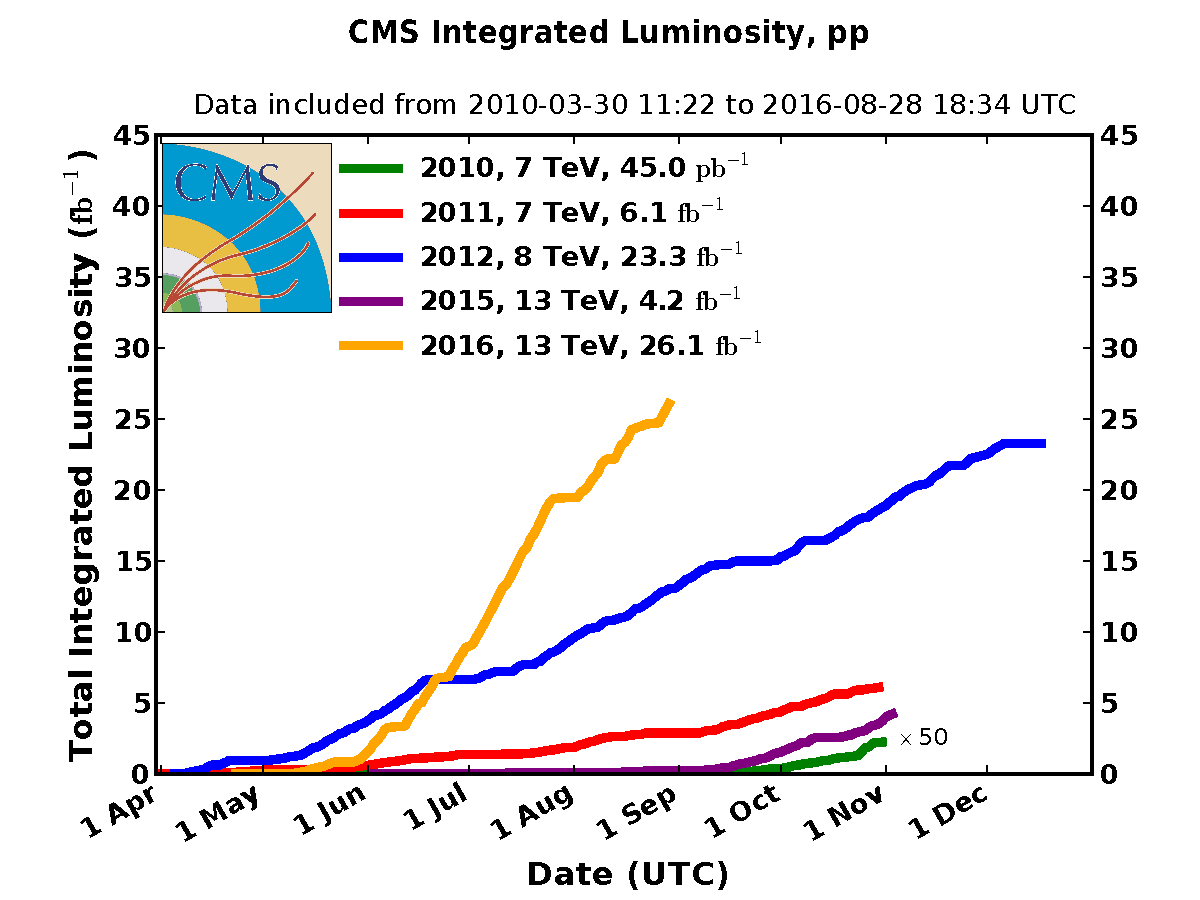
\includegraphics[width=1.0\columnwidth]{figures_chapter2/int_lumi_cumulative_pp_2}
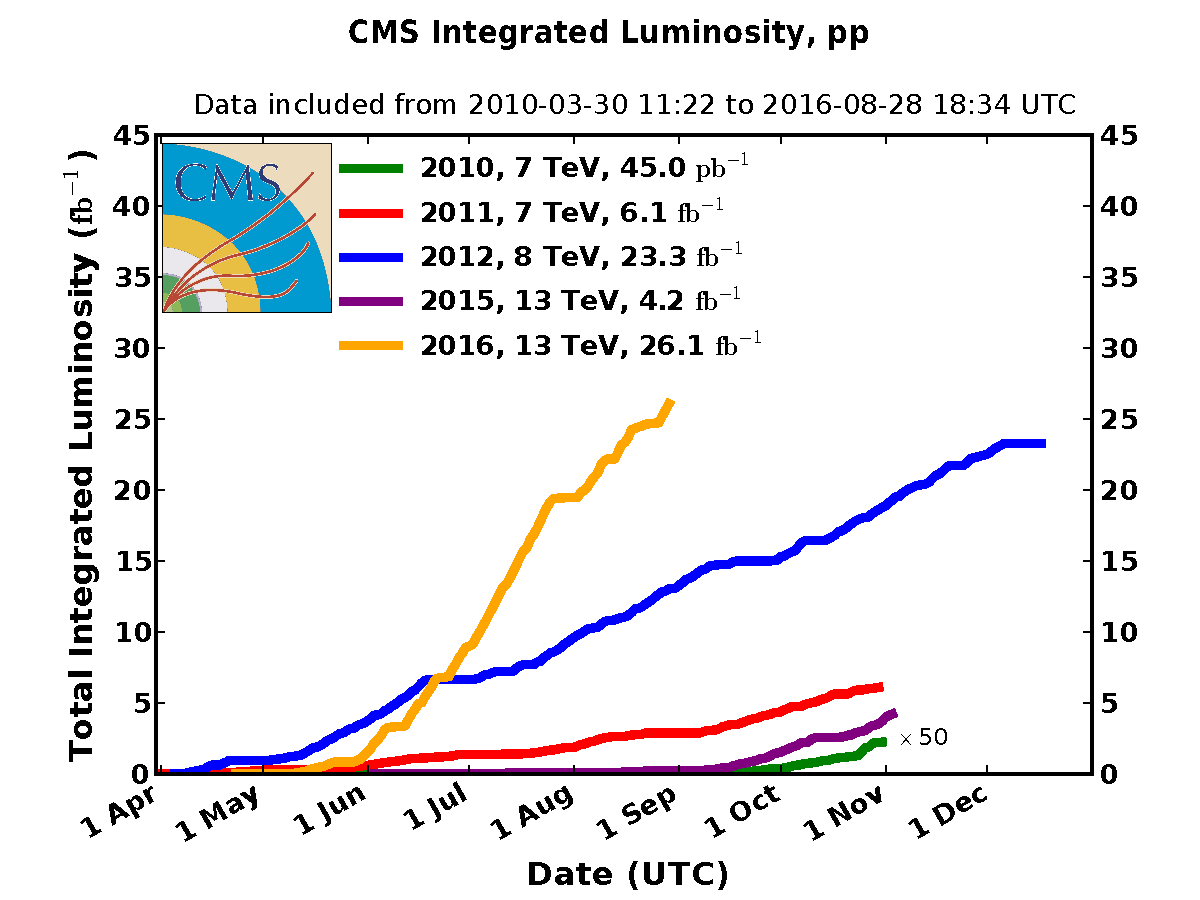
\includegraphics[width=0.8\columnwidth]{figures_chapter2/int_lumi_cumulative_pp_2}
\caption{The total integrated luminosity delivered to CMS during stable beams in proton-proton collisions~\cite{lumi_plot}. It is shown for $2010$ (green), $2011$ (red), $2012$ (blue), $2015$ (purple), and $2016$ (orange) data taking periods. The total integrated luminosity is shown for the data collected up to the end of August for the 2016 data taking period.} 
\label{fig:int}
\end{figure}

The machine luminosity depends only on the beam parameters. For a Gaussian beam distribution the dependance is given by
\begin{equation} \label{eq:lumi_beam}
L = \frac{N_{b}^2n_bf_{rev}\gamma_{r}}{4\pi\epsilon_n\beta^{*}}F,
\end{equation}
where $N_b$ is the number of particle per bunch ($\mathcal{O}(10^{11})$), $n_b$ is the number of bunches per beam, $f_{rev}$ is the revolution frequency, $\gamma_r$ is the relativistic gamma factor, $\epsilon_n$ is the normalized transverse beam emittance, $\beta^{*}$ is the beta function at the collision point, and $F$ is the geometric luminosity reduction factor due to the crossing angle at the interaction point.  The LHC has four interaction points that host ALICE~\cite{Aamodt:2008zz}, ATLAS~\cite{Aad:2008zzm}, CMS~\cite{Chatrchyan:2008aa}, and LHCb~\cite{Alves:2008zz} detectors. The ATLAS and CMS are general purpose, high luminosity experiments. The LHCb is a forward detector specializing in heavy flavor physics. The ALICE experiment is designed to study heavy-ion collisions.   

Figure~\ref{fig:int} shows the total integrated luminosity delivered to CMS during stable beams from October, $2010$ to August, $2016$ data taking periods. The LHC delivered proton-proton collisions at $\sqrt{s}$ of $7~\TeV$ during $2010$ and $2011$. The total integrated luminosity delivered in $2011$ was $6.1~\ifb$ with a peak instantaneous luminosity of $4.0 \times 10^{33}$ cm$^2$ s$^{-1}$. The luminosity recorded and certified, where all the detector sub-components are confirmed to operate normally, for physics results was $5.1~\ifb$. $\sqrt{s}$ was increased to $8~\TeV$ in $2012$ with $23.3~\ifb$ total integrated luminosity delivered to CMS with a peak instantaneous luminosity of $7.7 \times 10^{33}$ cm$^2$ s$^{-1}$. The total certified data amounted to $19.7~\ifb$. A bunch spacing of $50$ ns was used in the $2011$ and $2012$ data taking periods. 

\begin{figure}[h]
\centering
%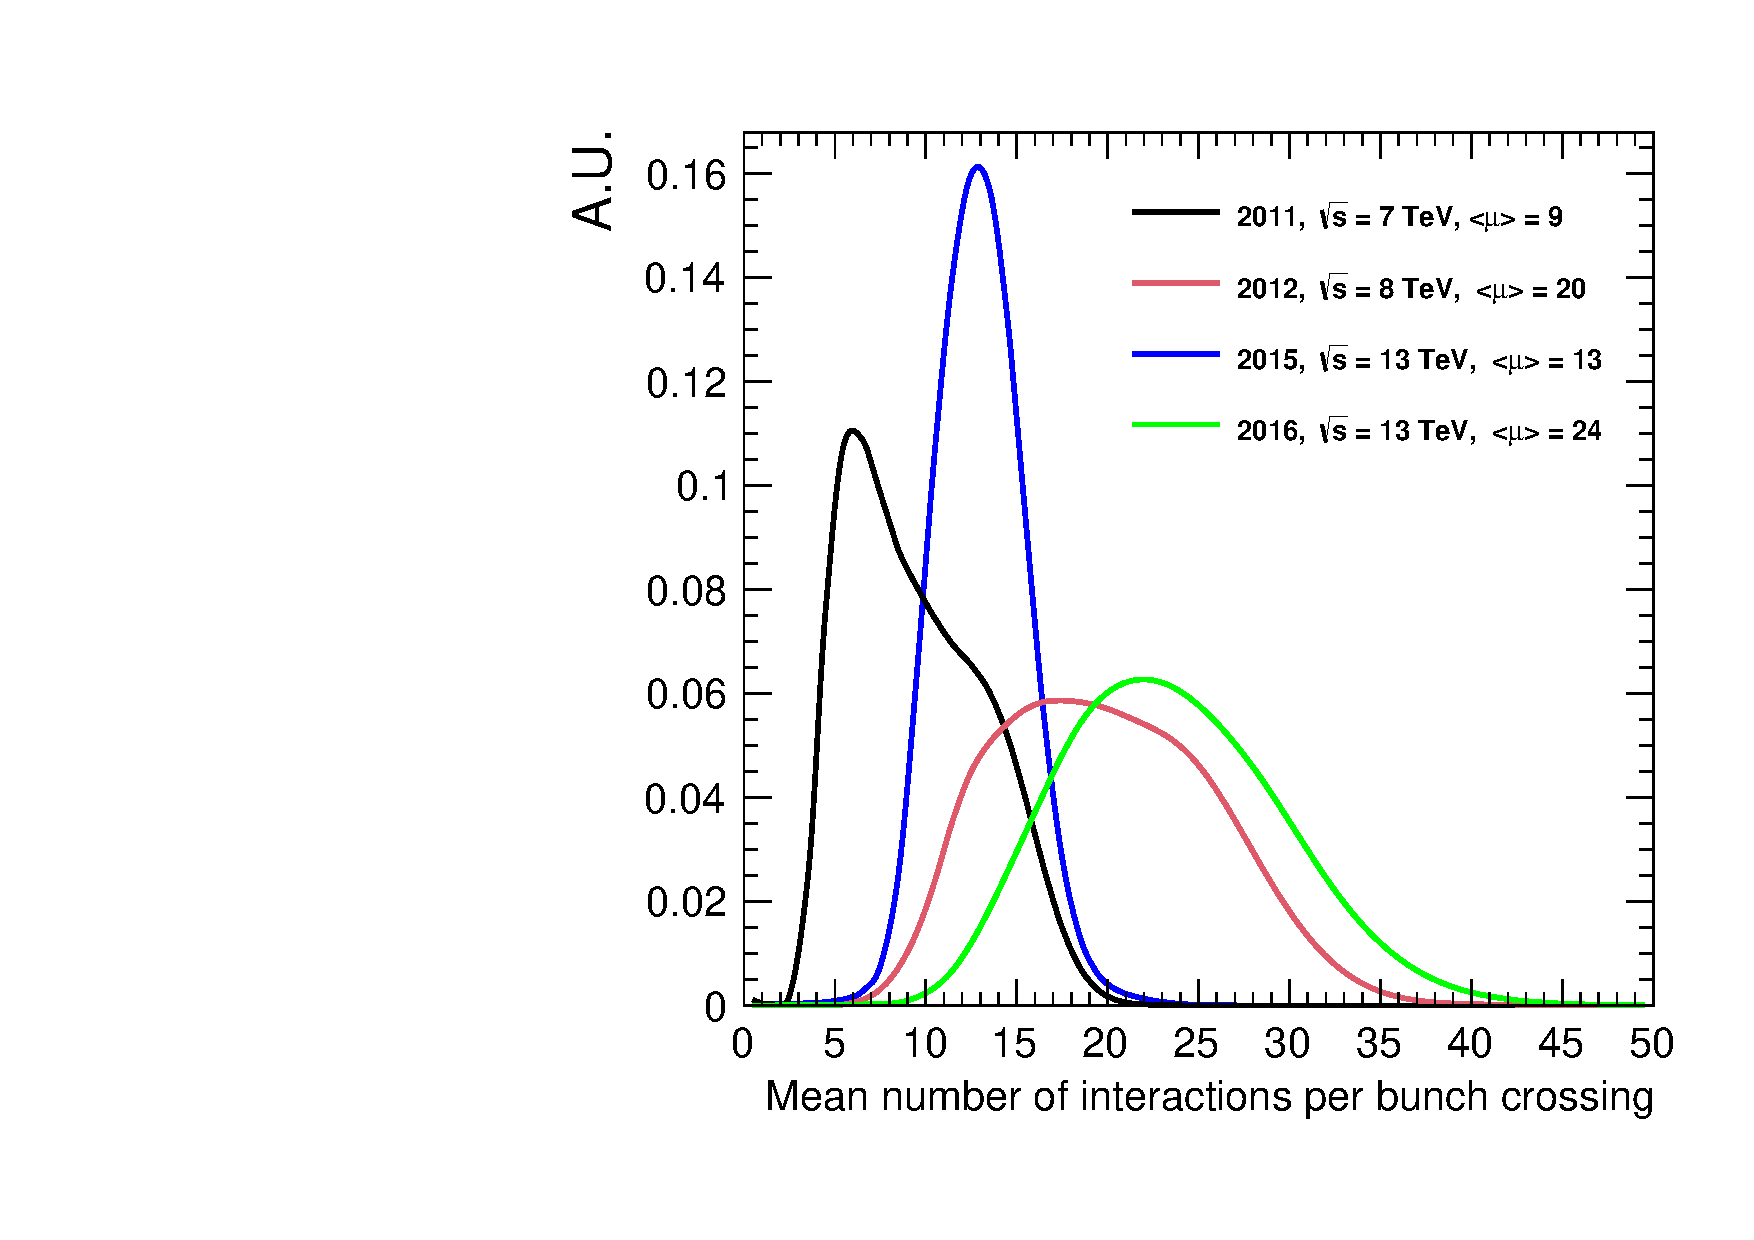
\includegraphics[width=1.0\columnwidth]{figures_chapter2/pileup_cms}
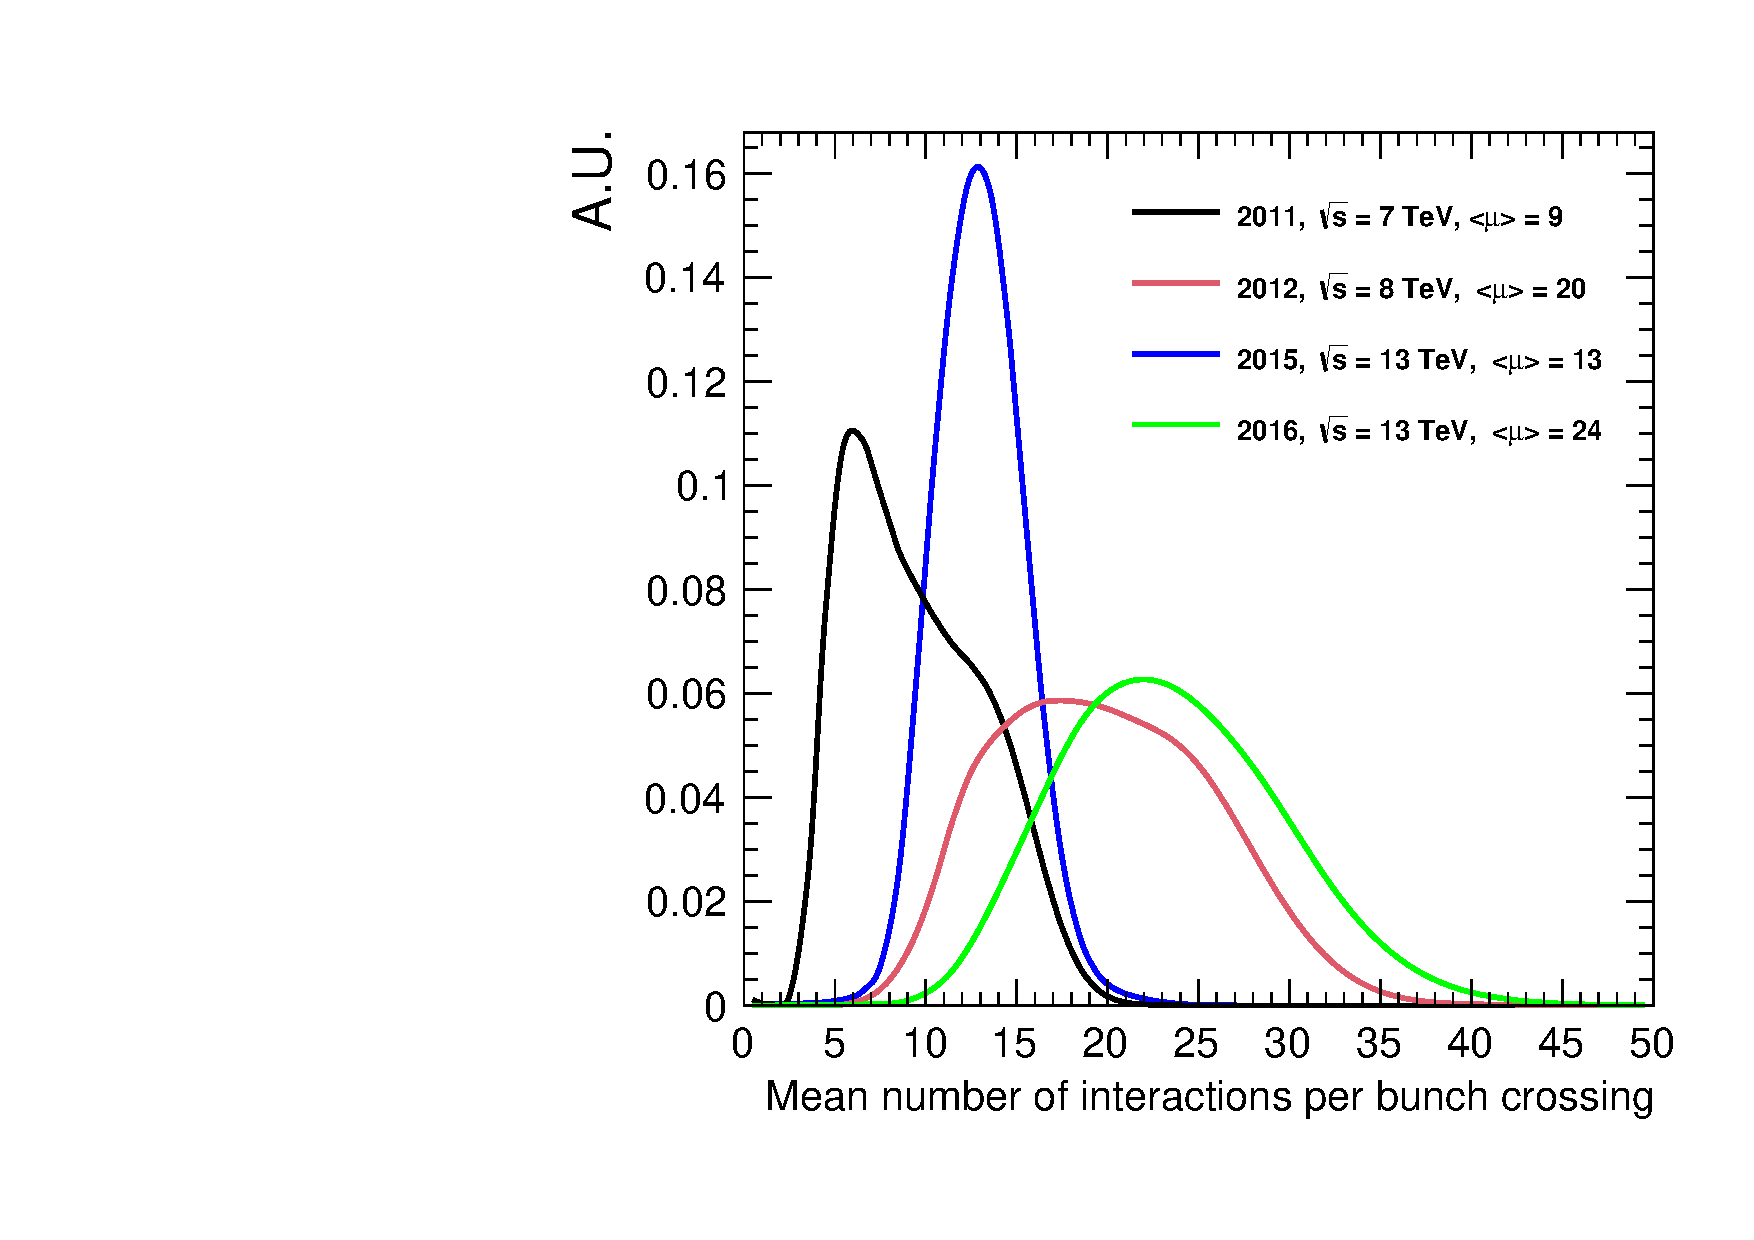
\includegraphics[width=0.6\columnwidth]{figures_chapter2/pileup_cms}
\caption{Mean number of interactions per bunch crossing in proton-proton collisions. A detailed description of the  luminosity measurements in CMS can be found here~\cite{CMS-PAS-LUM-13-001,CMS-PAS-LUM-15-001}. The distributions are shown for $2011$ (black), $2012$ (red), $2015$ (blue), and $2016$ (green) data taking periods.}
\label{fig:pu}
\end{figure} 

The LHC entered the Long Shutdown $1$ (LS1) in $2013$ for maintenance and upgrades during which the CMS detector was upgraded as well. The data taking resumed in $2015$ with $4.2~\ifb$ total integrated luminosity delivered to CMS with a peak instantaneous luminosity of $5.1 \times 10^{33}$ cm$^2$ s$^{-1}$. The LHC started to operate with the nominal bunch spacing of $25$ ns during this period. The total certified data for the nominal CMS operation and bunch spacing of $25$ ns amounted to $2.3~\ifb$. The data taking continued in $2016$ with an excellent performance by the LHC with significantly lower transverse beam sizes. This was achieved using a new bunch production scheme which resulted in a peak luminosity of  $1.2 \times 10^{34}$ cm$^2$ s$^{-1}$. Total integrated luminosity of $26.1~\ifb$ was delivered by the end of August of $2016$.   

Figure~\ref{fig:pu} shows the mean number of additional inelastic proton-proton interactions per bunch crossing (pileup). The additional pileup interactions in events present challenges in reconstruction and identification of the particles originating from the hard scattering of interest. The average number of pileup interactions in $2011$ was $9$ as the instantaneous luminosity continuously increased during the year. The average number of pileup interactions further increased to $20$ in $2012$ and reached to $24$ during $2016$.  While higher instantaneous luminosities are desired to enhance the production of the events of interest, the effects of pileup need to be mitigated to improve the sensitivity of the results. 

\section{Proton-Proton Collisions and Event Simulation}

The $W$, $Z$, and Higgs bosons are produce via the interactions of the quarks and gluons (referred as partons) inside the protons of the LHC colliding proton beams~\cite{Bloom:1969kc,Breidenbach:1969kd}. The cross section of a given process is given by:
\begin{eqnarray} \label{eq:xsec}
\begin{aligned}
\sigma_{p_ap_b \rightarrow n} &= \sum_{a,b} \int dx_a dx_b f_{a/A}(x_a,\mu_{F}^2) f_{b/B}(x_{b},\mu_{F}^2)  \\ 
& \times [\hat{\sigma}_{LO}(x_ax_bs,\mu_R^2,\mu_F^2)+\alpha_s(\mu_R^2)\hat{\sigma}_{NLO}(x_ax_bs,\mu_R^2,\mu_F^2)+...],
\end{aligned}
\end{eqnarray}   
where $f_{a/A}$, $f_{b/B}$ are the parton distribution functions (PDF) for the quarks and gluons inside the proton, $x_i$ is the relative parton momentum in the direction of proton (Bjorken-$x$), and $\hat{\sigma}$ denote the parton-parton cross section at the centre-of-mass energy $x_{a}x_{b}s$, where $s$ is the squared of the proton-proton centre-of-mass energy.  This is illustrated in Figure~\ref{fig:lhc_collision} for the $Z$ boson production. The PDFs can not be described through perturbative calculations however the collinear factorization theorem can be applied to separate the perturbative and non-perturbative regimes in Eq.~(\ref{eq:xsec})~\cite{Collins:1989gx}. The scale at which this separation happens is denoted as the factorization scale $\mu_{F}$. The basic idea is to absorb the large logarithms appearing in the calculations due to collinear emissions of the parton into the PDFs. This scale dependance of the PDFs is described by the Dokshitzer-Gribov-Lipatov-Altarelli-Parisi (DGLAP) parton evolution equations allowing to evolve a given PDF parametrization to a desired scale~\cite{Gribov:1972ri,Altarelli:1977zs,Dokshitzer:1977sg}. In this way parameterized functional forms are fitted to data and then evolved to a scale of interest by solving the DGLAP equations either in leading-order, next-to-leading-order (NLO) or NNLO. PDF fits by several collaborations are used in the results.

\begin{figure}[h]
\centering
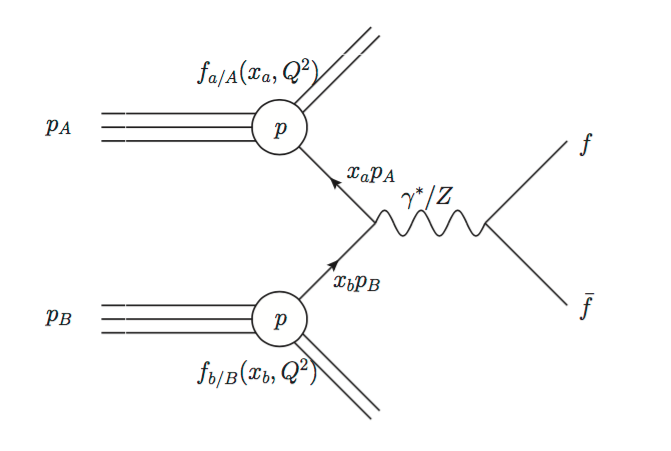
\includegraphics[width=0.60\columnwidth]{figures_chapter2/lhc_cross}
\caption{Illustration of the $Z$ boson production in proton-proton collisions. The parton momenta are given by $x_ap_a$ and $x_bp_b$~\cite{Schott:2014sea}.}
\label{fig:lhc_collision}
\end{figure} 

The matrix elements (ME) needed to evaluate the partonic cross sections are performed using a Monte Carlo (MC) sampling to integrate the phase space. The QCD ME calculations are done up to a fixed number of final state partons. The transverse momenta of the bosons are zero at LO calculations. The real emissions in the higher order QCD corrections can explain the observed $p_{T}$ distributions of the $W$ and $Z$ bosons for example (there is also a very small boson $p_{T}$ due to a small transverse momentum of the parton inside the proton). Thus the measurement of the $p_{T}$ distributions of these bosons provides new constraints to understand the higher order QCD (and electroweak) corrections. At small vector boson $p_{T}$ large logarithmic corrections appear in the fixed order calculations due to collinear gluon emissions. These logarithmic corrections due to these emissions cancel with the virtual corrections for the inclusive calculations. Resummation can be carried out to provide accurate predictions of the vector boson $p_{T}$ at the low values of the $p_T$~\cite{Laenen:1991af}.

ME calculations at fixed orders break down for soft momenta and collinear final state partons. Parton shower models are used to evolve the partons from the hard scales to the non-perturbative hadron scales. The parton showers are modeled as a sequence os branchings $q \rightarrow qg$, $g \rightarrow q\bar{q}$, and $g \rightarrow g g$ in QCD and $q \rightarrow q\gamma$ and $\ell \rightarrow \ell \gamma$ in quantum electrodynamics (QED) where $q$, $g$, $\ell$, and $\gamma$ denote a quark, gluon, lepton, and photon respectively~\cite{Schott:2014sea}. The branchings from the initial and final partons add additional outgoing partons in the event. It has to be noted that unlike the ME approach the parton method does not include the spin effects. 

The parton showering is continued up to the scale $\Lambda_{QCD} \approx 200~\MeV$. The final partons are hadronized into color-neutral hadrons to obtain the full generated event simulation. The models are tuned to the data. The unstable hadrons (traveling less than few mm) are decayed according to the branching ratios. Additional parton-parton interactions in the colliding protons, known as multi-parton interactions (MPI), are included as well. The specific software tools utilized to generate the events used in the results are referenced in chapter $4$.  

\section{The $W$,$Z$, and Higgs boson productions at the LHC}

The production of the electroweak gauge bosons at the LHC proton-proton collisions proceeds mainly via the Drell-Yan process~\cite{Drell:1970wh}. At least one sea quark is required to produce the gauge bosons in the proton-proton collisions and it is dominated by $u\bar{d} \rightarrow W^{+}$, $d\bar{u} \rightarrow W^{-}$, and $u\bar{u},d\bar{d} \rightarrow Z$. The relations between the mass $M$ and rapidity $y$ of the vector boson and the kinematics of the colliding partons are given by:
\begin{eqnarray} \label{eq:kinematics}
\begin{aligned}
M^2 &= x_{1}x_{2}s, \\
y &= \frac{1}{2} \mathrm{ln}\left(\frac{E+p_{z}}{E-p_{z}}\right) = \frac{1}{2}\mathrm{ln}\left(\frac{x_1}{x_2}\right), \\
x_{1/2} &= \frac{M}{\sqrt{s}} \mathrm{exp}(\pm y).
\end{aligned}
\end{eqnarray}   
This is illustrated in Figure~\ref{fig:lhc_grid}. Hence for the $W$ and $Z$ boson production with masses of $\mathcal{O} (100~\GeV)$ and rapidity $|y|<2.5$ the Bjorken-$x$ values are in the range of $10^{-3}$ to $0.1$. Theoretical predictions of the inclusive $W$ and $Z$ production cross sections are available at NNLO in perturbative QCD~\cite{Rijken:1994sh,Hamberg:1990np,vanNeerven:1991gh,Harlander:2002wh,PhysRevD.69.094008}. The precision of the predictions is limited by the uncertainties in PDFs and higher order QCD and EWK corrections. The energy scale of the process means that the sea quarks in the protons are mainly due to the gluon splitting $g \rightarrow q\bar{q}$ and therefore the uncertainty of the gluon PDFs plays a role as well.

\begin{figure}[h]
\centering
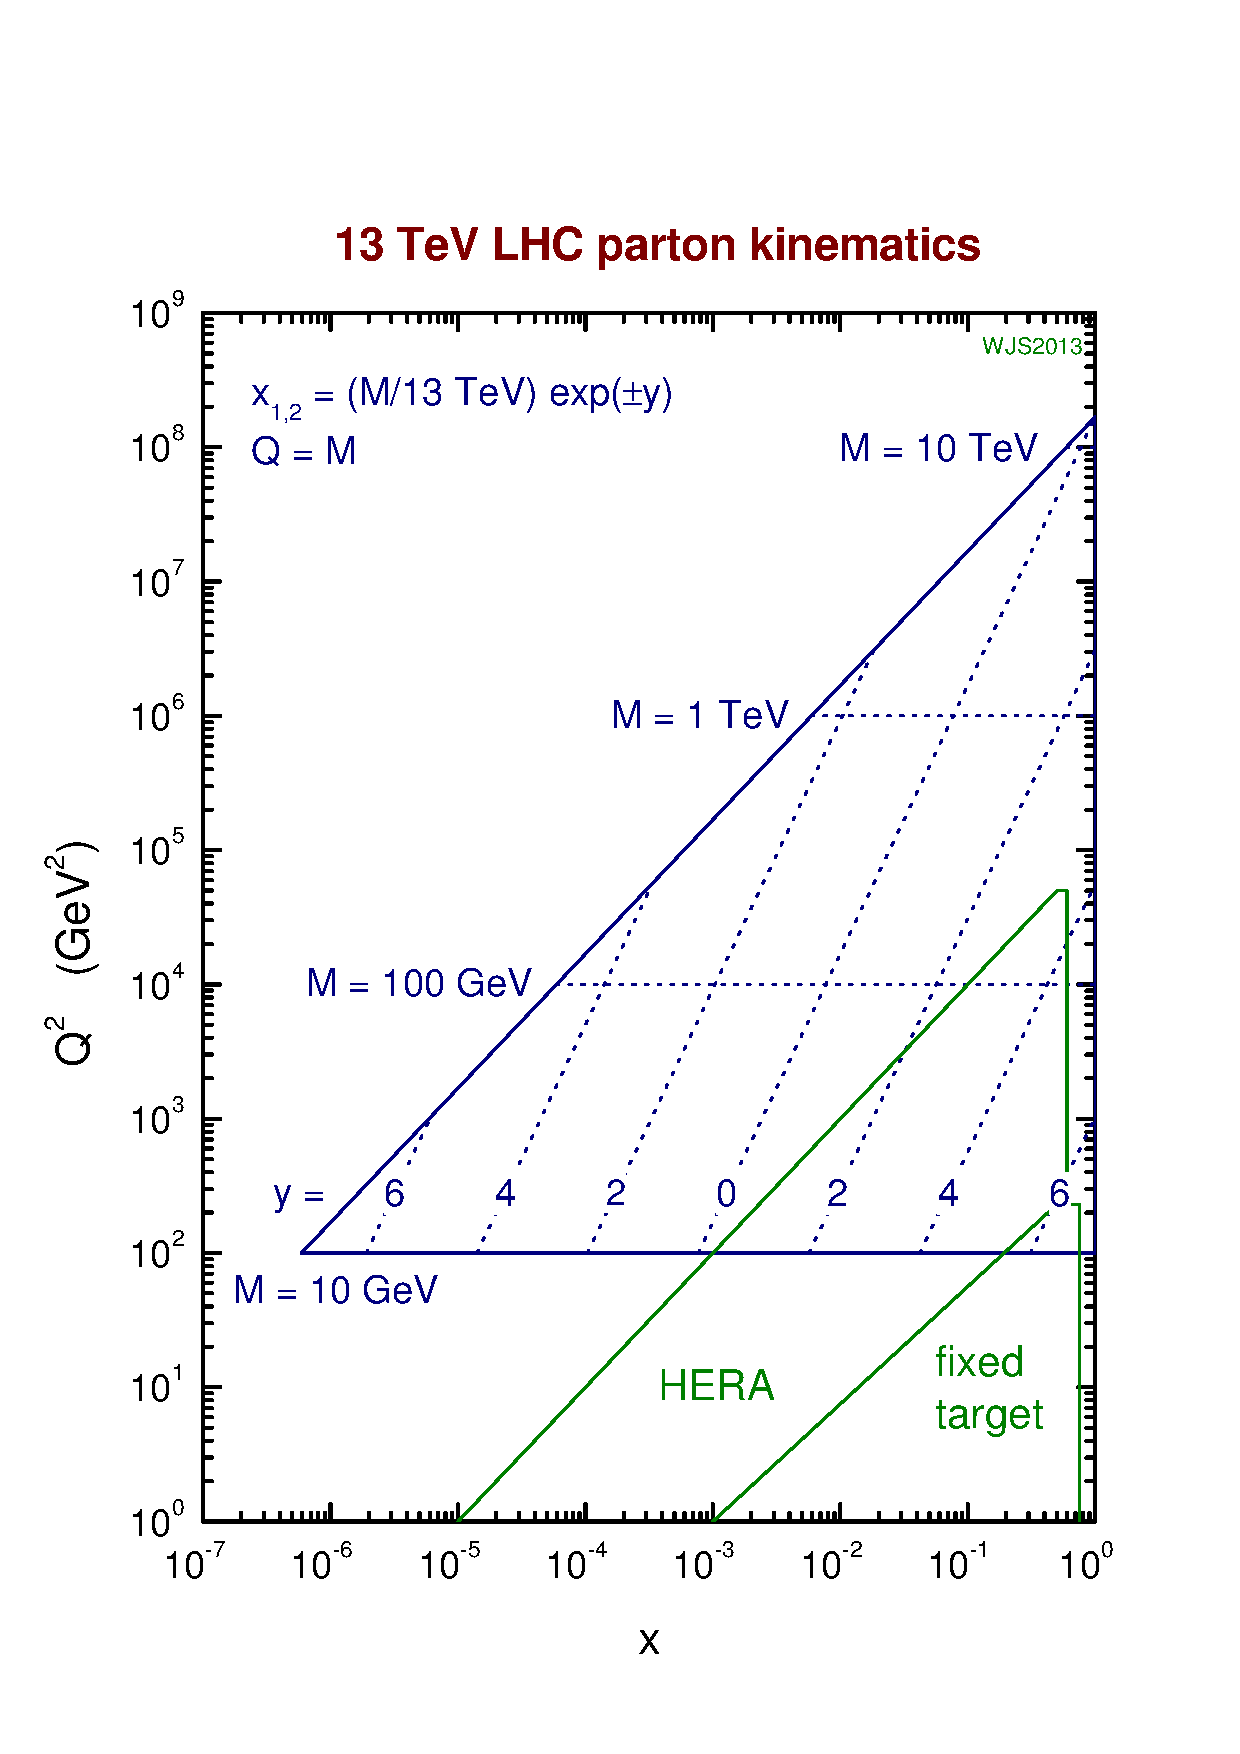
\includegraphics[width=0.49\columnwidth]{figures_chapter2/lhcgrid13}
\caption{Available kinematic plane in Bjorken-$x$ and the scale of the process $Q^2$ at the LHC centre-of-mass energy $\sqrt{s}=13~\TeV$. $M$ and $y$ are the mass and rapidity of the final state parton. The corresponding plane for the deep inelastic experiments is shown in green~\cite{sterling}. }
\label{fig:lhc_grid}
\end{figure} 

The leptonic decays of the $W$ and $Z$ bosons provide a large dataset of relatively pure and isolated leptonic events. $Z \rightarrow \ell \ell$ events can be used to calibrate the detector as well as the stability of the luminosity measurement of the proton-proton collisions. The inclusive total cross section measurements and ratios test the perturbative higher order corrections and constrain the PDFs of the protons. The importance of the higher order QCD corrections on the boson transverse momenta distribution was discussed in the last section. Better understanding of these effects allows to make precise measurements of the fundamental electroweak parameters such as the mass of the $W$ boson and the electroweak mixing angle. In addition, the $W$ and $Z$ boson production is a background source for the SM Higgs boson studies and many BSM physics searches.

\begin{figure}[h]
\centering
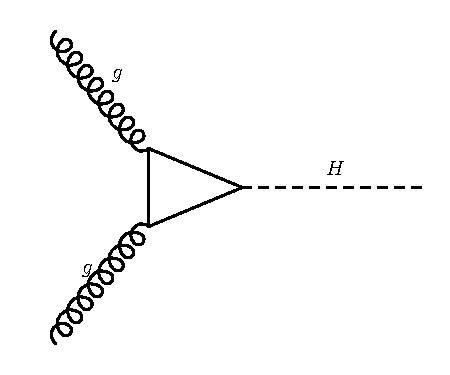
\includegraphics[width=0.49\columnwidth]{figures_chapter2/g_fusion}
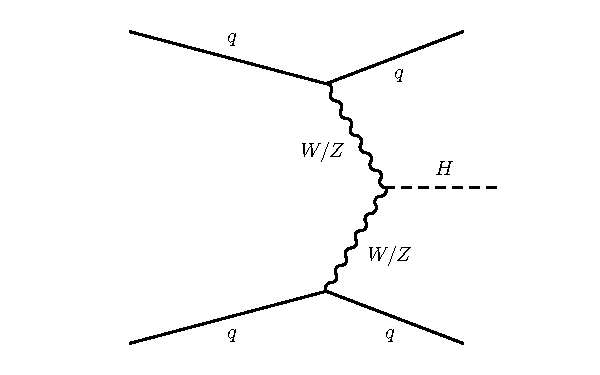
\includegraphics[width=0.49\columnwidth]{figures_chapter2/vbf}
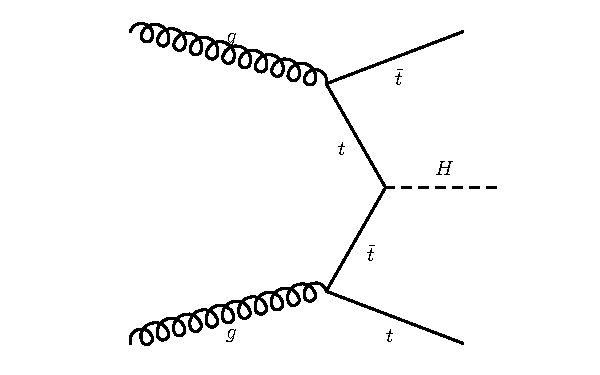
\includegraphics[width=0.49\columnwidth]{figures_chapter2/tth}
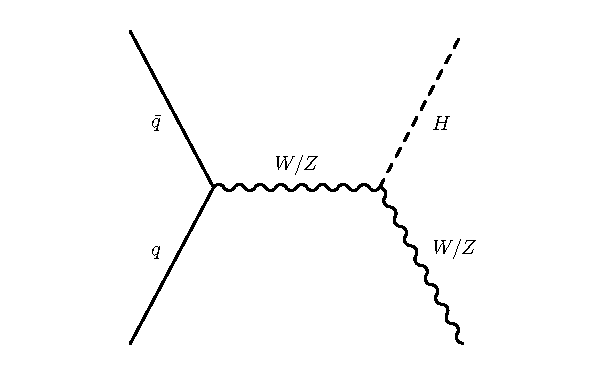
\includegraphics[width=0.49\columnwidth]{figures_chapter2/vh}
\caption{Leading order Feynman diagrams contributing to the SM Higgs boson production at the LHC in gluon fusion (top left), vector boson fusion (top right), Higgsstrahlung (bottom left), and top quark associated production (bottom right). }
\label{fig:sm_higgs}
\end{figure} 

Figure~\ref{fig:sm_higgs} shows the main leading order Ferynman diagrams contributing to the SM Higgs boson production at the LHC. The gluon fusion production, where the Higgs is produced from an intermediate quark loop, is the dominant mode~\cite{Georgi:1977gs}. It is dominated by the top quark loop as the Higgs coupling to fermions is proportional to the mass of the fermion in question. The Vector Boson Fusion (VBF) production~\cite{Cahn:1983ip}, where the Higgs boson is produced from an intermediate $W/Z$ bosons radiated from the colliding quarks, has an interesting experimental signature that can be exploited.  The VBF produced Higgs events are produced in association with two high energy forward jets (the jets are discussed in chapter $3$) in the opposite regions of the detector.  There is typically very little hadronic activity in the central region of the detector as there is no "color flow" between the quarks. Higgsstrahlung~\cite{Glashow:1978ab}, where the Higgs boson is radiated from a $W$ or $Z$ boson produced in $s$ channel at leading order, is the next largest Higgs boson production mode.  The Higgs bosons produced in VBF and Higgsstrahlung processes tend to have higher transverse momenta compared to Higgs bosons produced in the gluon fusion mode. The Higgs boson can also be produced in association with a top and anti-top pair~\cite{Raitio:1978pt,Ng:1983jm,Kunszt:1984ri,Marciano:1991qq}.There are other Higgs production modes, not relevant for the current Higgs boson studies, that will be important to consider at higher integrated luminosities at the LHC. The SM Higgs boson production cross sections are shown in Figure~\ref{fig:higgs_cross} as a function of the Higgs boson mass at $\sqrt{s}=8~\TeV$ and as a function of $\sqrt{s}$ for the Higgs mass of $125~\GeV$. The individual cross sections for the four Higgs boson production mechanisms discussed above are shown. The calculations are done up to NNLO in QCD and NLO in EWK~\cite{Dittmaier:2011ti,Dittmaier:2012vm,Heinemeyer:2013tqa}. The gluon fusion predictions are also resummed to next-nto-ntext to leading logarithmic (NNLL) accuracy. The total production cross section is $22.3$ pb at   at $\sqrt{s}=8~\TeV$ and $50.6$ pb at $\sqrt{s}=13~\TeV$ for the Higgs mass of $125~\GeV$.  Recent calculations to $N^{3}LO$ in QCD for the gluon fusion~\cite{Anastasiou:2016cez} and VBF production modes~\cite{Dreyer:2016oyx} have become available. 

\begin{figure}[ht]
\centering
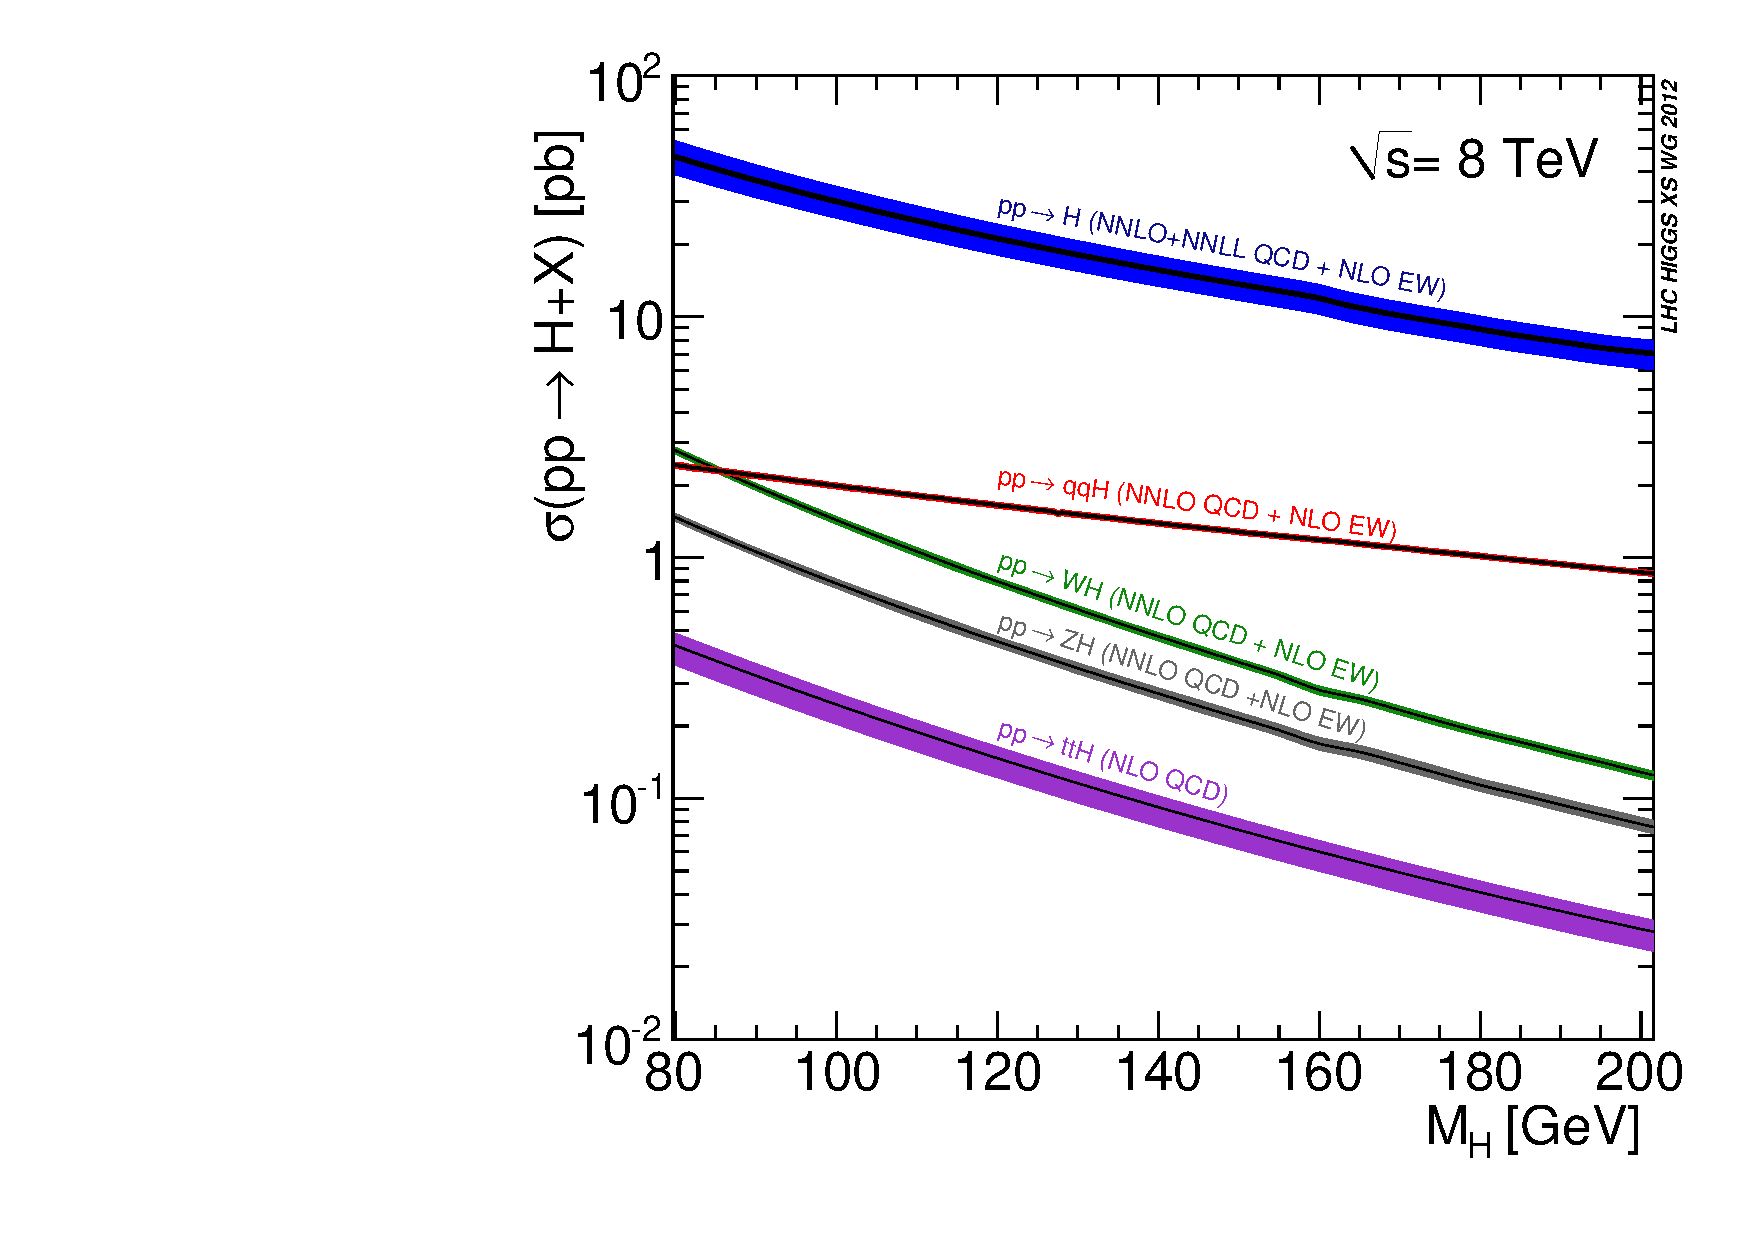
\includegraphics[width=0.49\columnwidth]{figures_chapter2/Higgs_XS_8TeV_LM200}
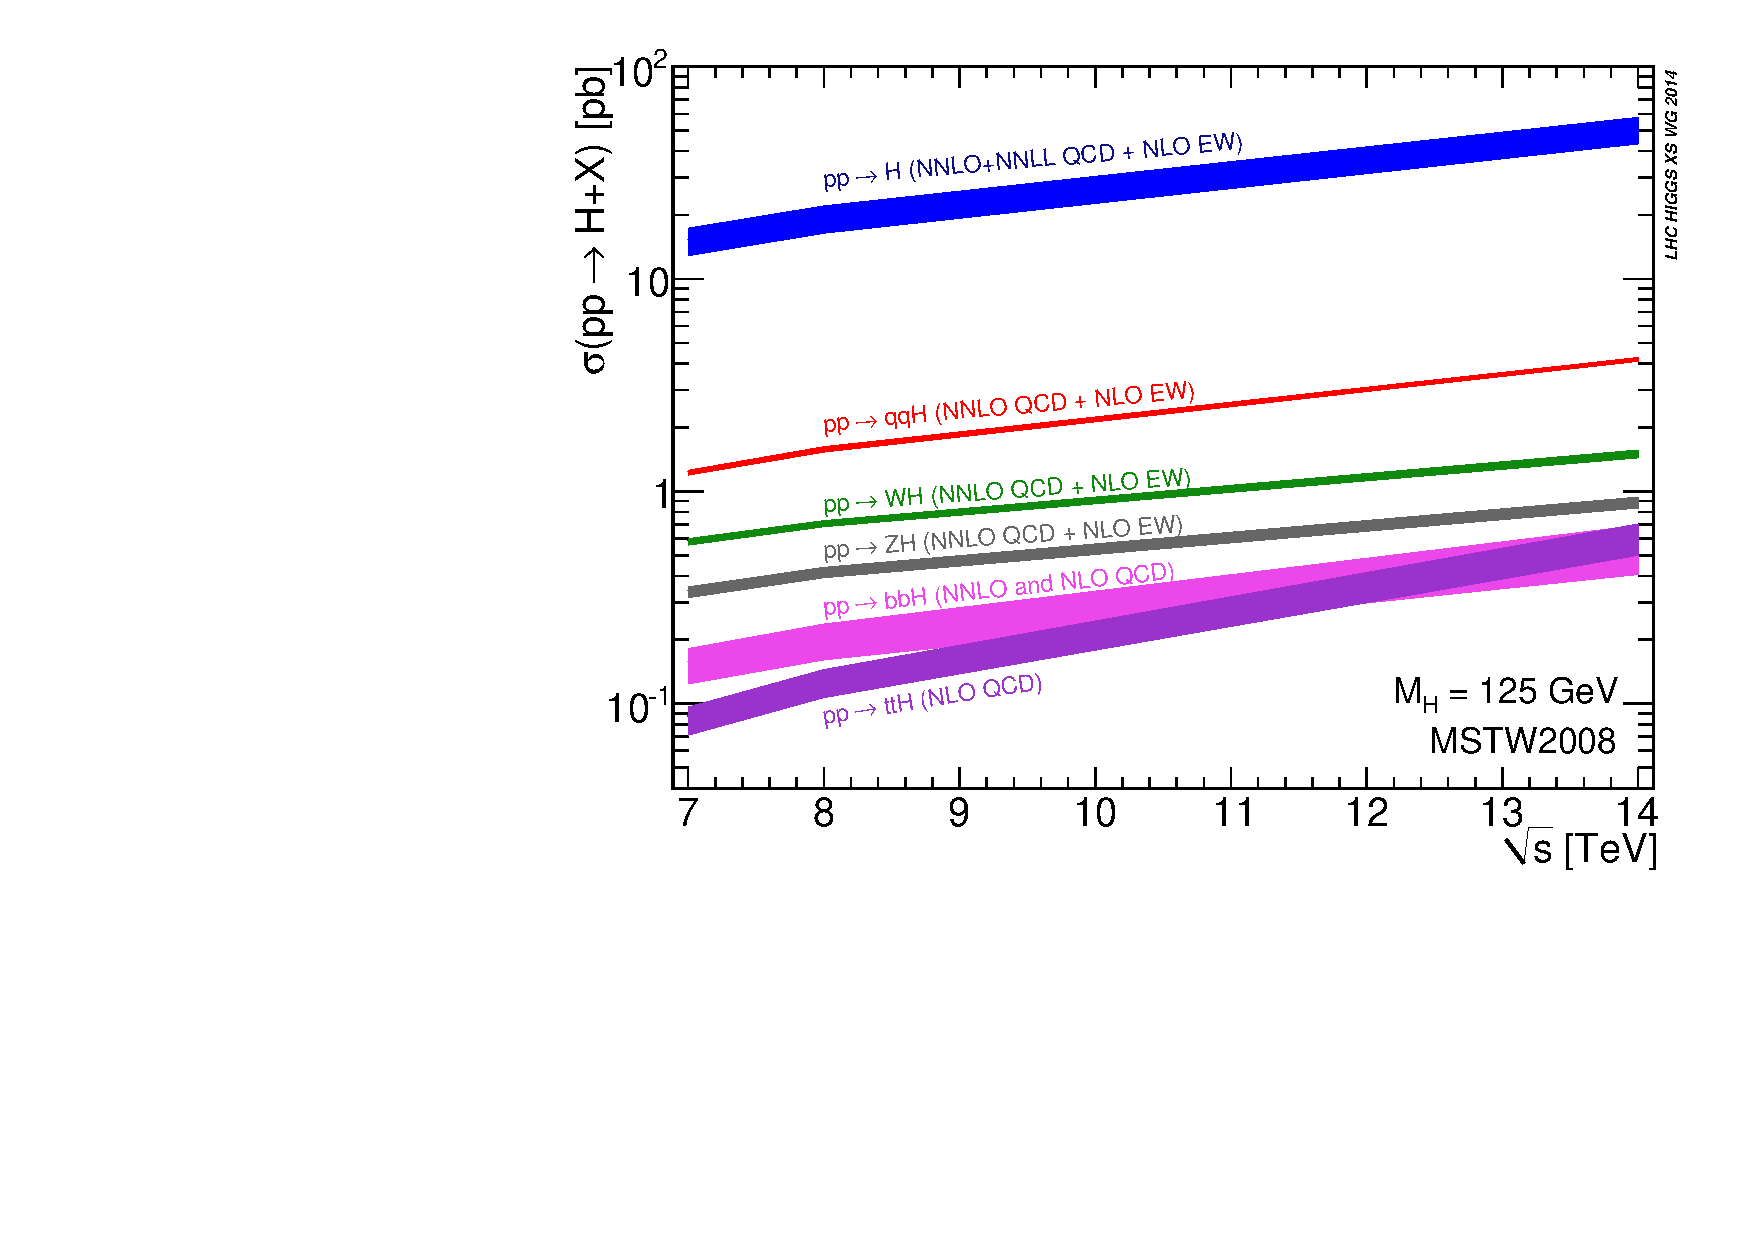
\includegraphics[width=0.49\columnwidth]{figures_chapter2/7-14}
\caption{Higgs boson production cross sections for the different production modes as a function of the Higgs mass at $\sqrt{s}=8~\TeV$ (left panel) and centre-of-mass energy $\sqrt{s}$ for the Higgs mass of $125~\GeV$ (right panel)~\cite{Dittmaier:2011ti,Dittmaier:2012vm,Heinemeyer:2013tqa}.}
\label{fig:higgs_cross}
\end{figure} 

The SM Higgs branching fractions and the total width are shown as a function of the mass in Figure~\ref{fig:higgs_decay}. The total width is at the order of few $\MeV$ for the low Higgs masses. Higgs boson decays to $b\bar{b}$, $\tau\tau$ and $c\bar{c}$ are the dominating decay modes at very low Higgs mass as there is no phase space available for the Higgs boson decays to $W^{+}W^{-}$ and $ZZ$. Decays to $gg$, $\gamma\gamma$, and $Z\gamma$ are possible through loops. For the $\gamma\gamma$ and $Z\gamma$ mode there is an interference between the fermion and $W$ loops.  At the Higgs mass of $125~\GeV$ the branching ratio to the $\tau\tau$ decay channel is $0.063$.

\begin{figure}[h]
\centering
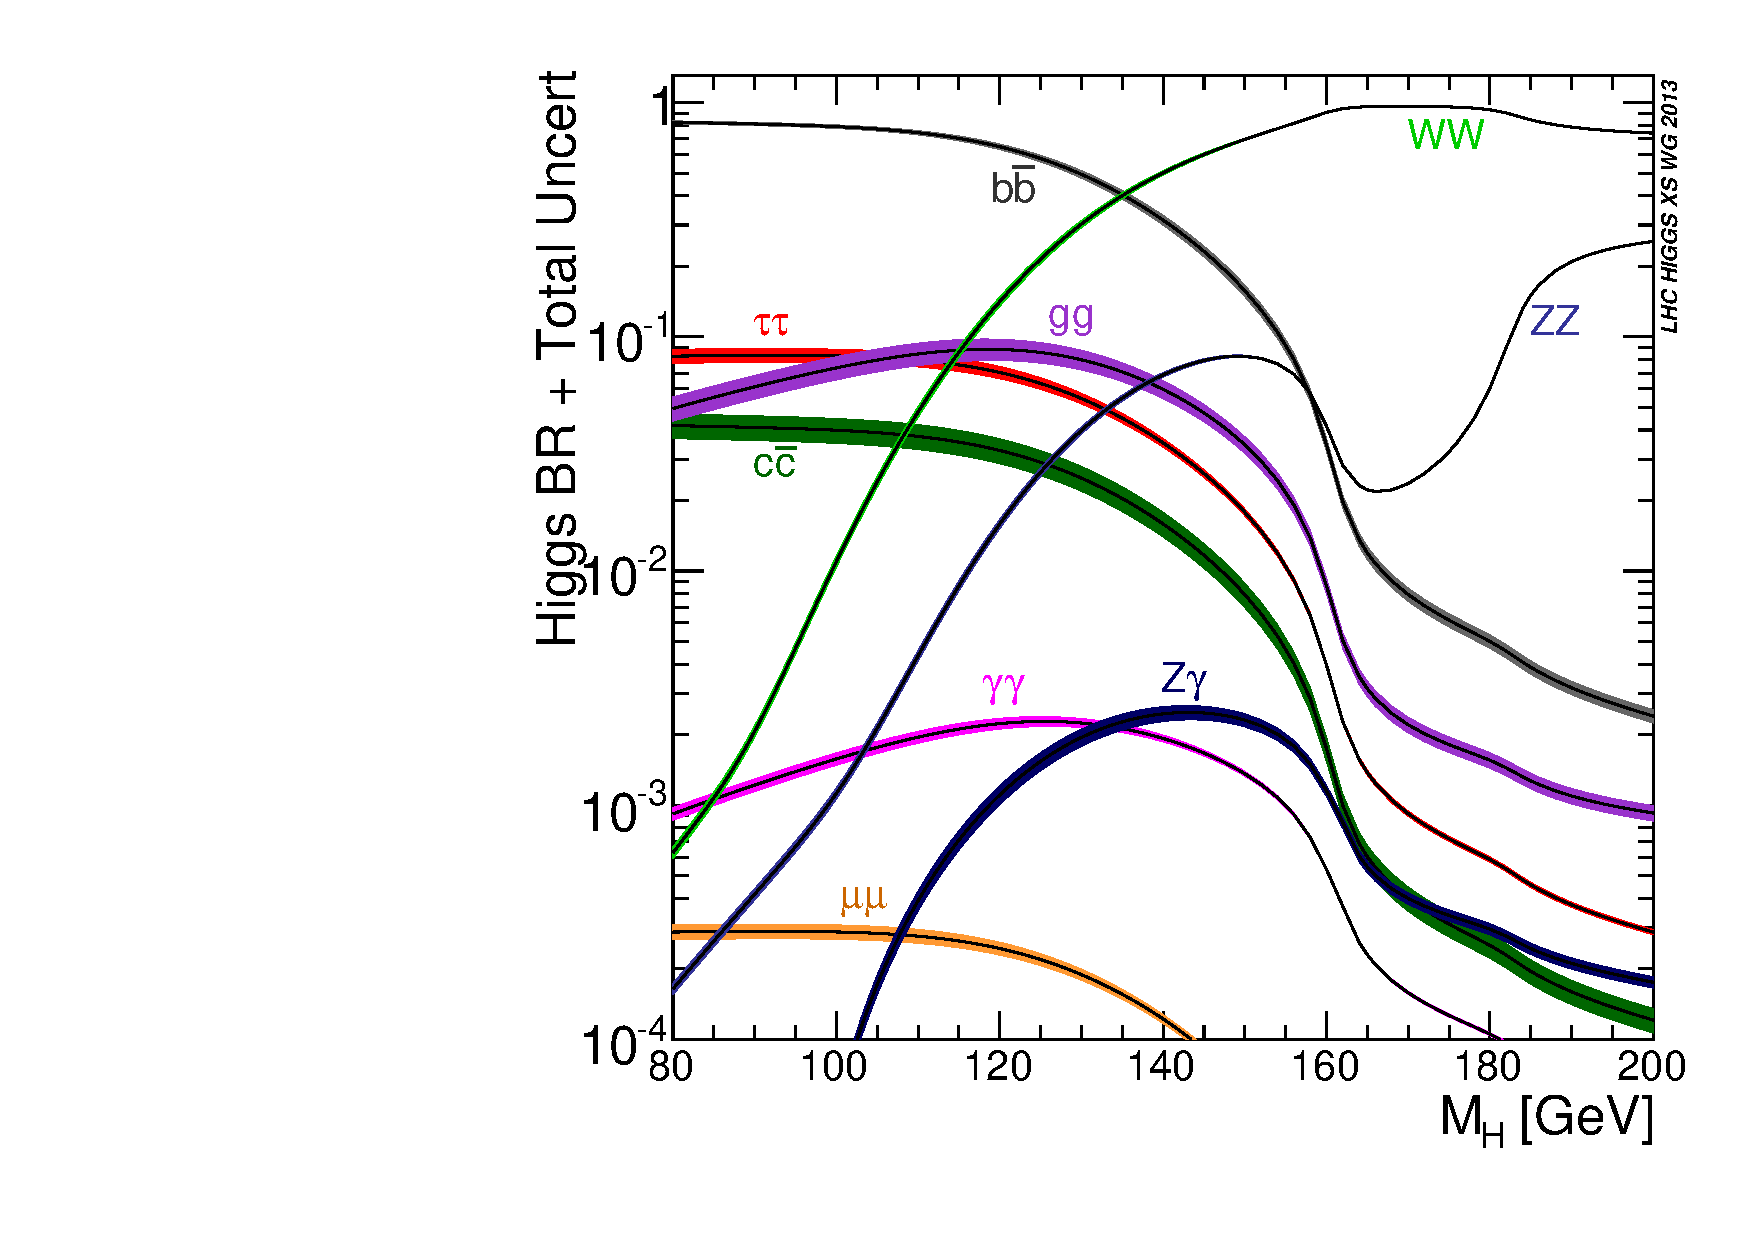
\includegraphics[width=0.49\columnwidth]{figures_chapter2/Higgs_BR_LM}
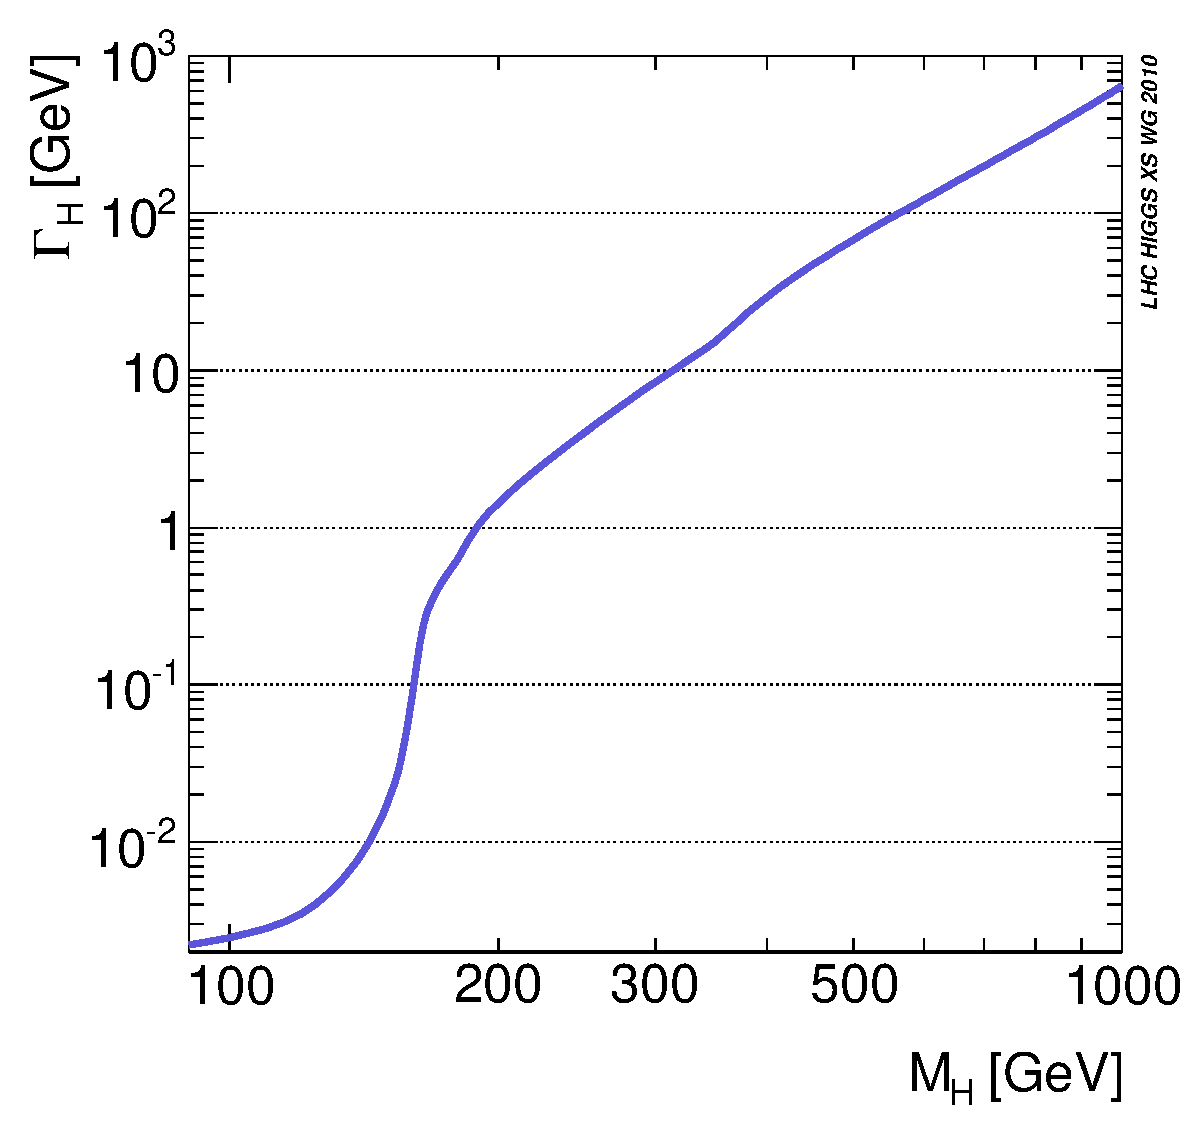
\includegraphics[width=0.49\columnwidth]{figures_chapter2/YRHXS_BR_fig2}
\caption{The largest Higgs boson branching ratios as a function (left panel) and total width as a function of the Higgs mass. The bands show the uncertainties in the branching fractions~\cite{Dittmaier:2011ti,Dittmaier:2012vm,Heinemeyer:2013tqa}.} 
\label{fig:higgs_decay}
\end{figure} 

It is possible to study the SM Higgs boson trilinear coupling by considering the Higgs pair-production as can be deduced from the Lagrangian in Eq.~(\ref{eq:ewk_higgs2})~\cite{Glover:1987nx,Plehn:1996wb,Djouadi:1999rca,Gianotti:2002xx,Baur:2003gpa,Baur:2003gp,Baglio:2012np}. This measurement would directly probe the potential of the Higgs field since the self-coupling is related to the third derivative of the Higgs potential at its minimum. The process is also sensitive to other BSM effects, as new physics can modify the rate of the production. Figure~\ref{fig:sm_dihiggs} shows the 
dominant Feynman diagrams for the gluon fusion production mode. Higgs boson pairs can be produced via a box diagram (left) and through the Higgs boson self-coupling contribution. The two processes interfere destructively. In fact the cross section is larger by a factor of two if only the box diagram is considered. The gluon fusion production cross section for the Higgs boson pair production has been calculated to NNLO~\cite{Dawson:1998py,Grigo:2014jma}. The cross section is $40.7$~fb at center-of-mass energy $\sqrt{s}=14~\TeV$. One can see that the SM Higgs boson pair production cross section is an order of magnitude smaller than the single Higgs boson production. Therefore, this process can be measured at the LHC only with very high integrated luminosities.

\begin{figure}[h]
\centering
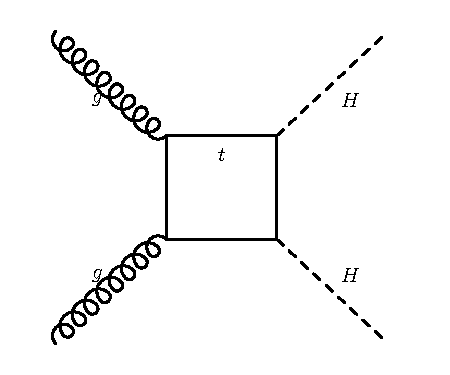
\includegraphics[width=0.49\columnwidth]{figures_chapter2/hhbox}
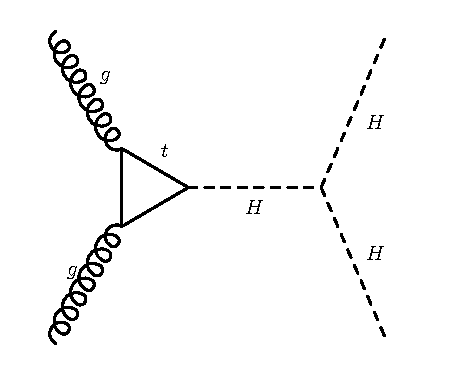
\includegraphics[width=0.49\columnwidth]{figures_chapter2/hhself}
\caption{Leading order Feynman diagrams contributing to the gluon fusion Higgs boson pair production at the LHC. The right diagram is the Higgs boson self-coupling contribution to the Higgs pair production.}
\label{fig:sm_dihiggs}
\end{figure} 


\begin{figure}[h]
\centering
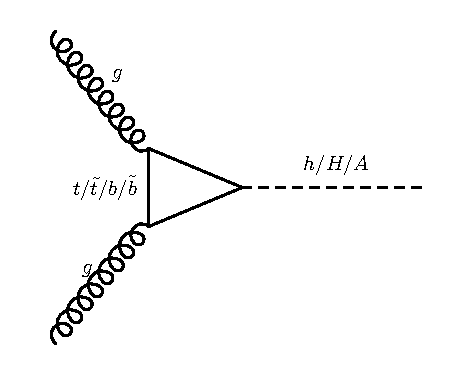
\includegraphics[width=0.49\columnwidth]{figures_chapter2/mssm_fusion}
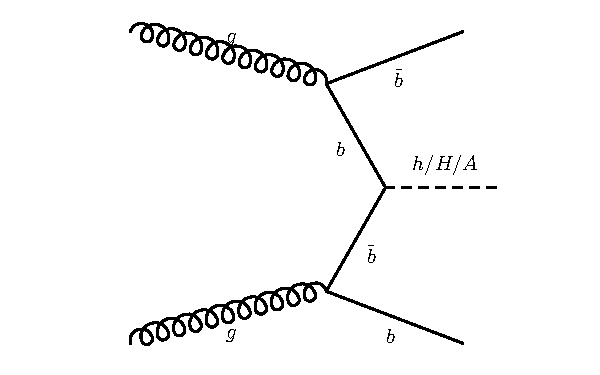
\includegraphics[width=0.49\columnwidth]{figures_chapter2/bbh_mssm}
\caption{Leading order Feynman diagrams contributing to the production of the MSSM Higgs bosons in gluon fusion (left) and b quark associated production (right).}
\label{fig:mssm_feynman}
\end{figure} 

\begin{figure}[h]
\centering
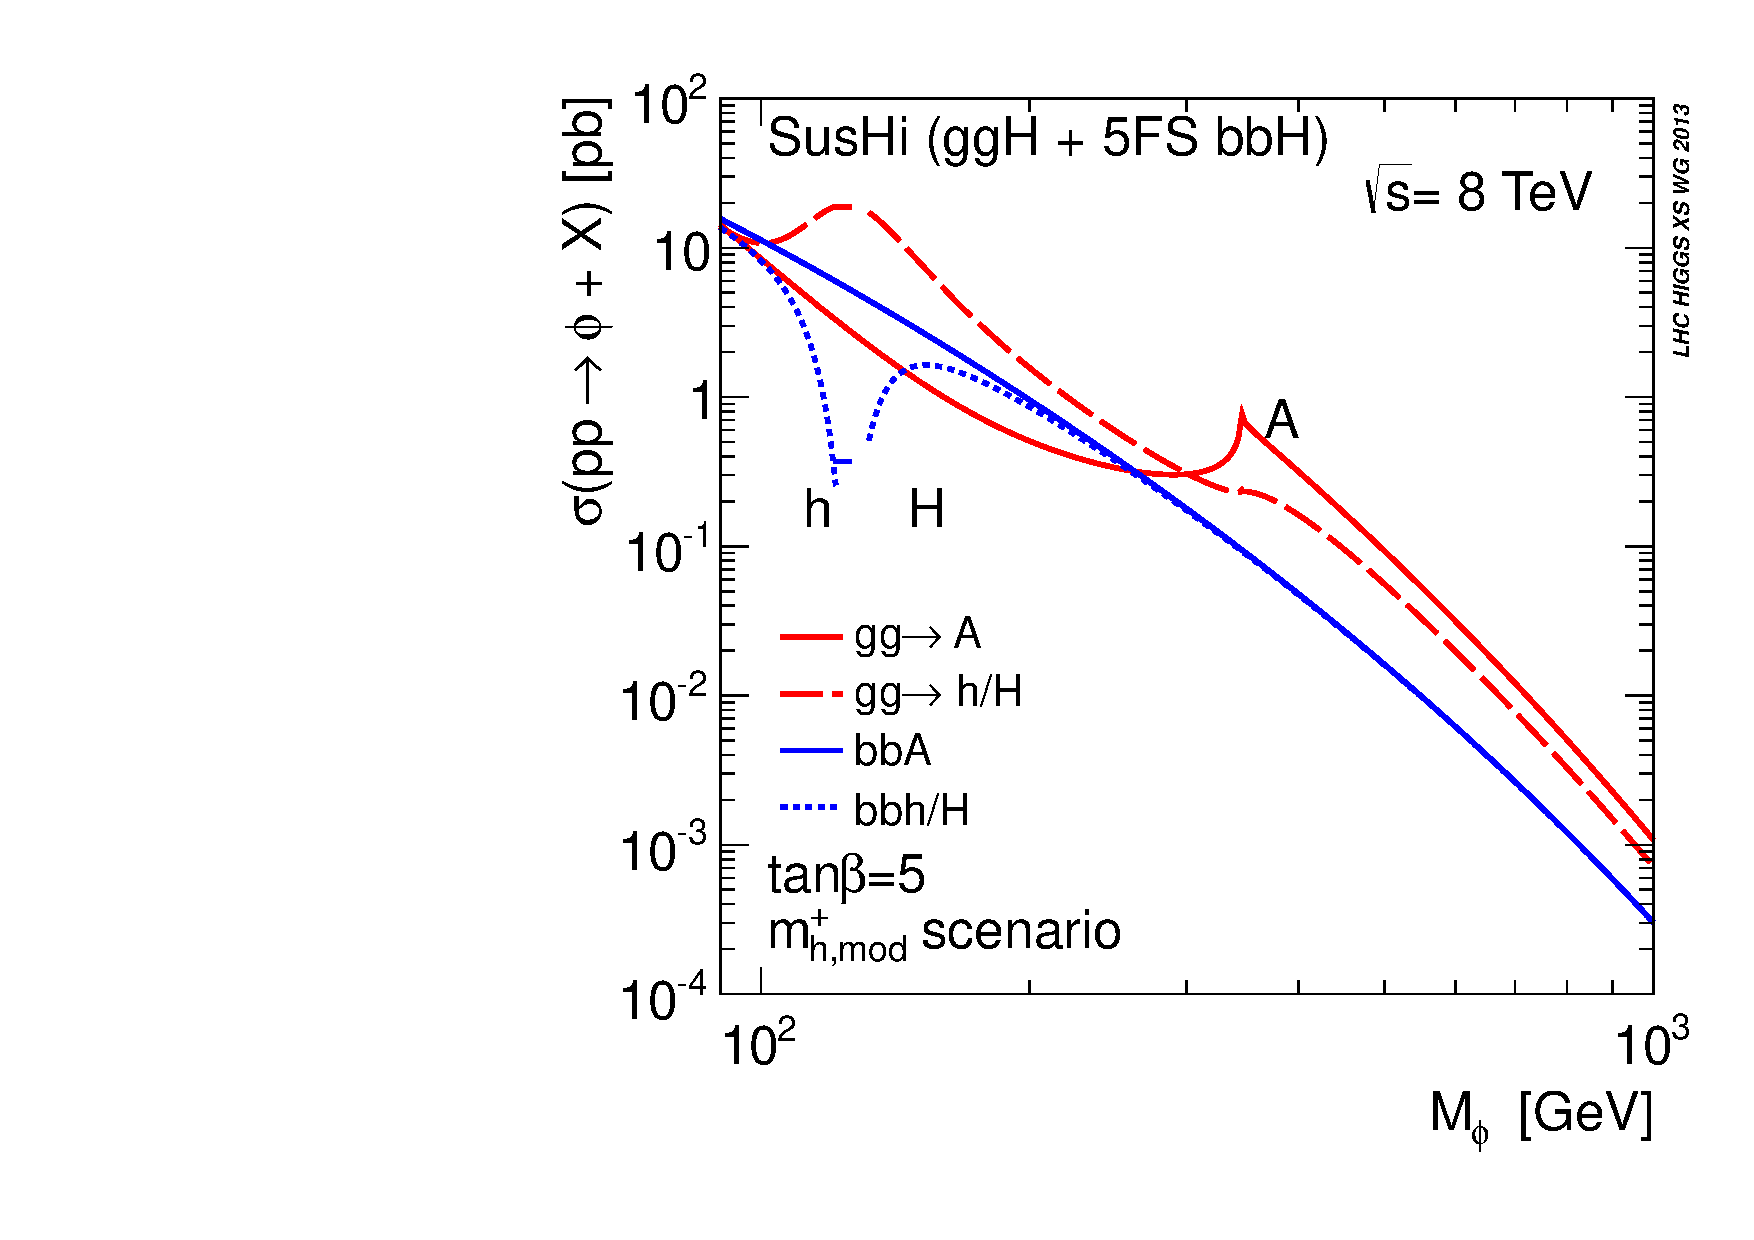
\includegraphics[width=0.49\columnwidth]{figures_chapter2/YR3HXS_XSectSummary_mhmodp_tanbeta5_SusHi}
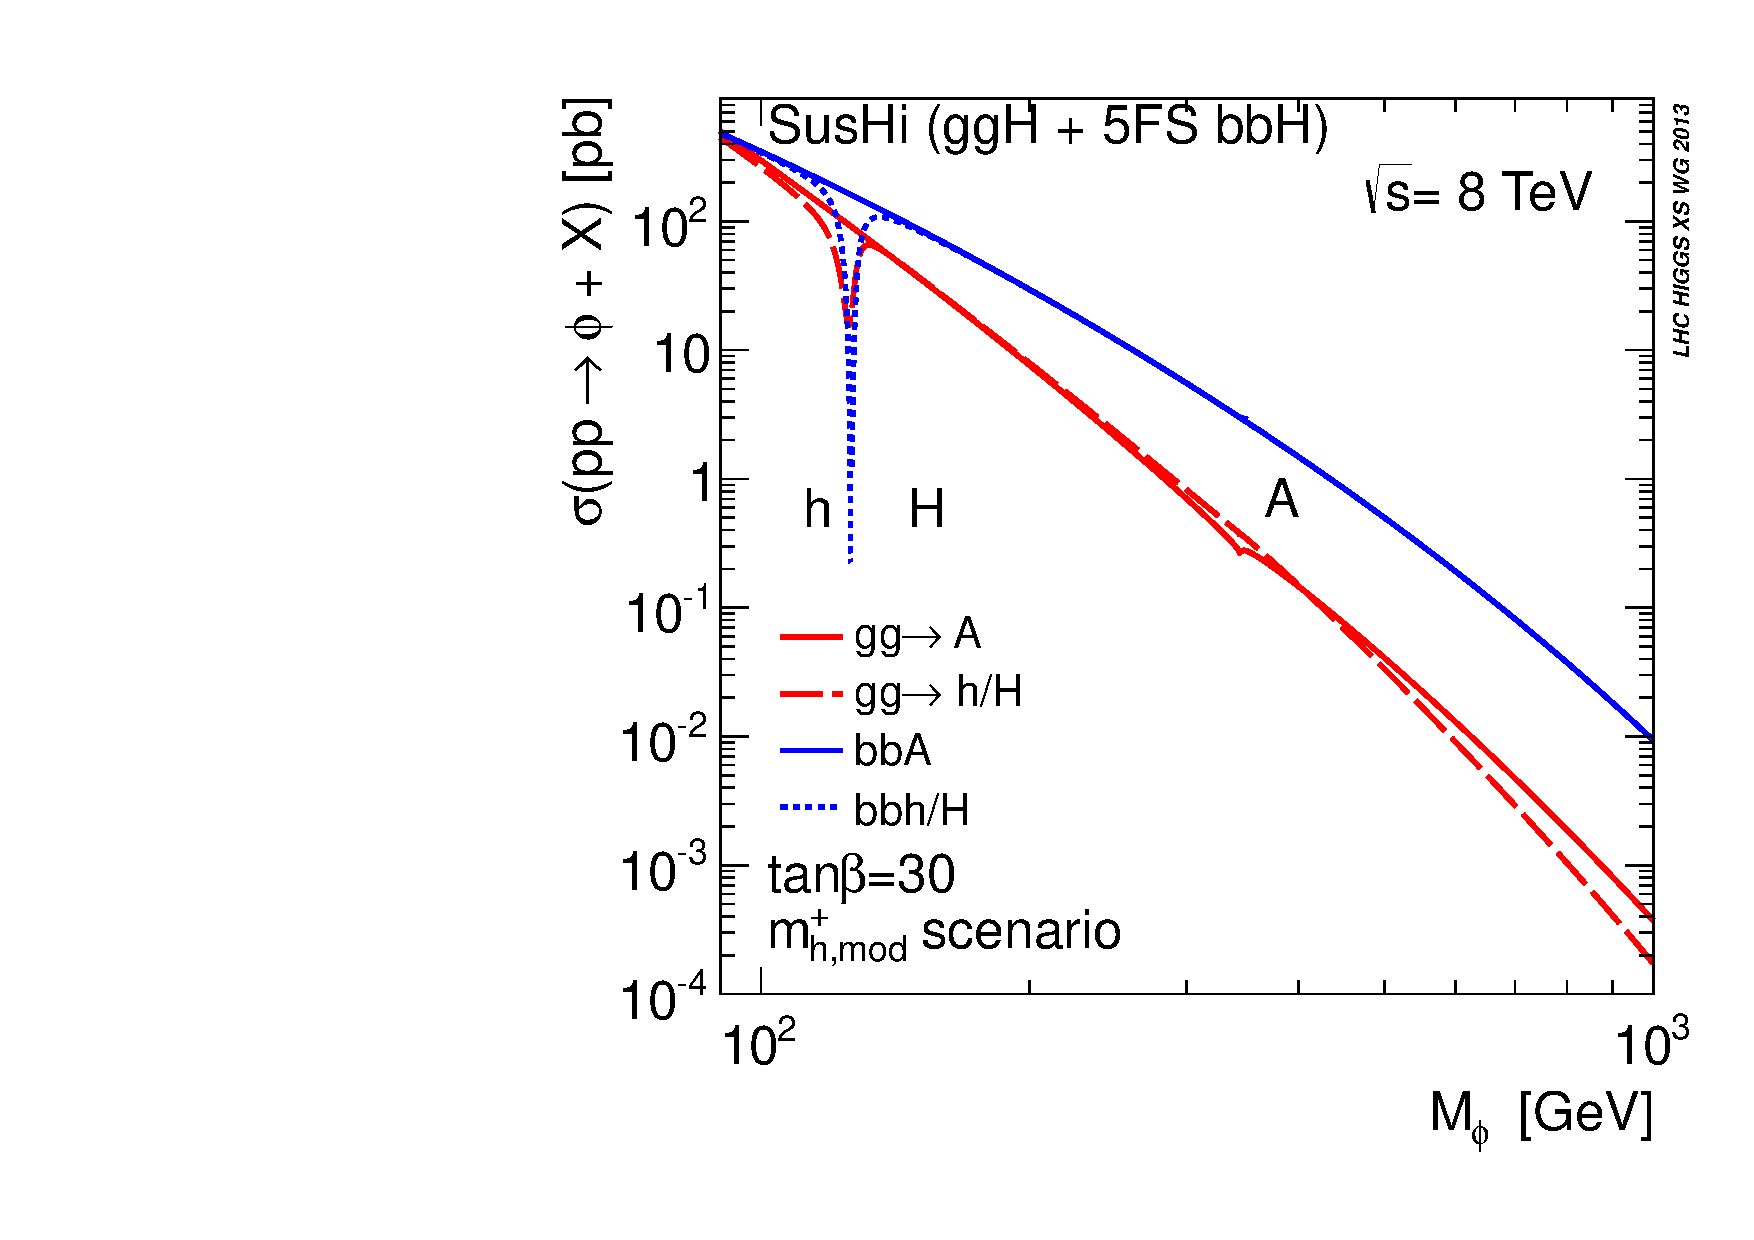
\includegraphics[width=0.49\columnwidth]{figures_chapter2/YR3HXS_XSectSummary_mhmodp_tanbeta30_SusHi}
\caption{Neutral Higgs boson production cross sections as a function of the CP-odd Higgs mass in the $m_{h}^{mod+}$ benchmark scenario with $\tan \beta = 5$ (left panel) and $\tan \beta = 30$ (right panel)~\cite{Dittmaier:2011ti,Dittmaier:2012vm,Heinemeyer:2013tqa}.} 
\label{fig:mssm_cross}
\end{figure} 

\begin{figure}[h]
\centering
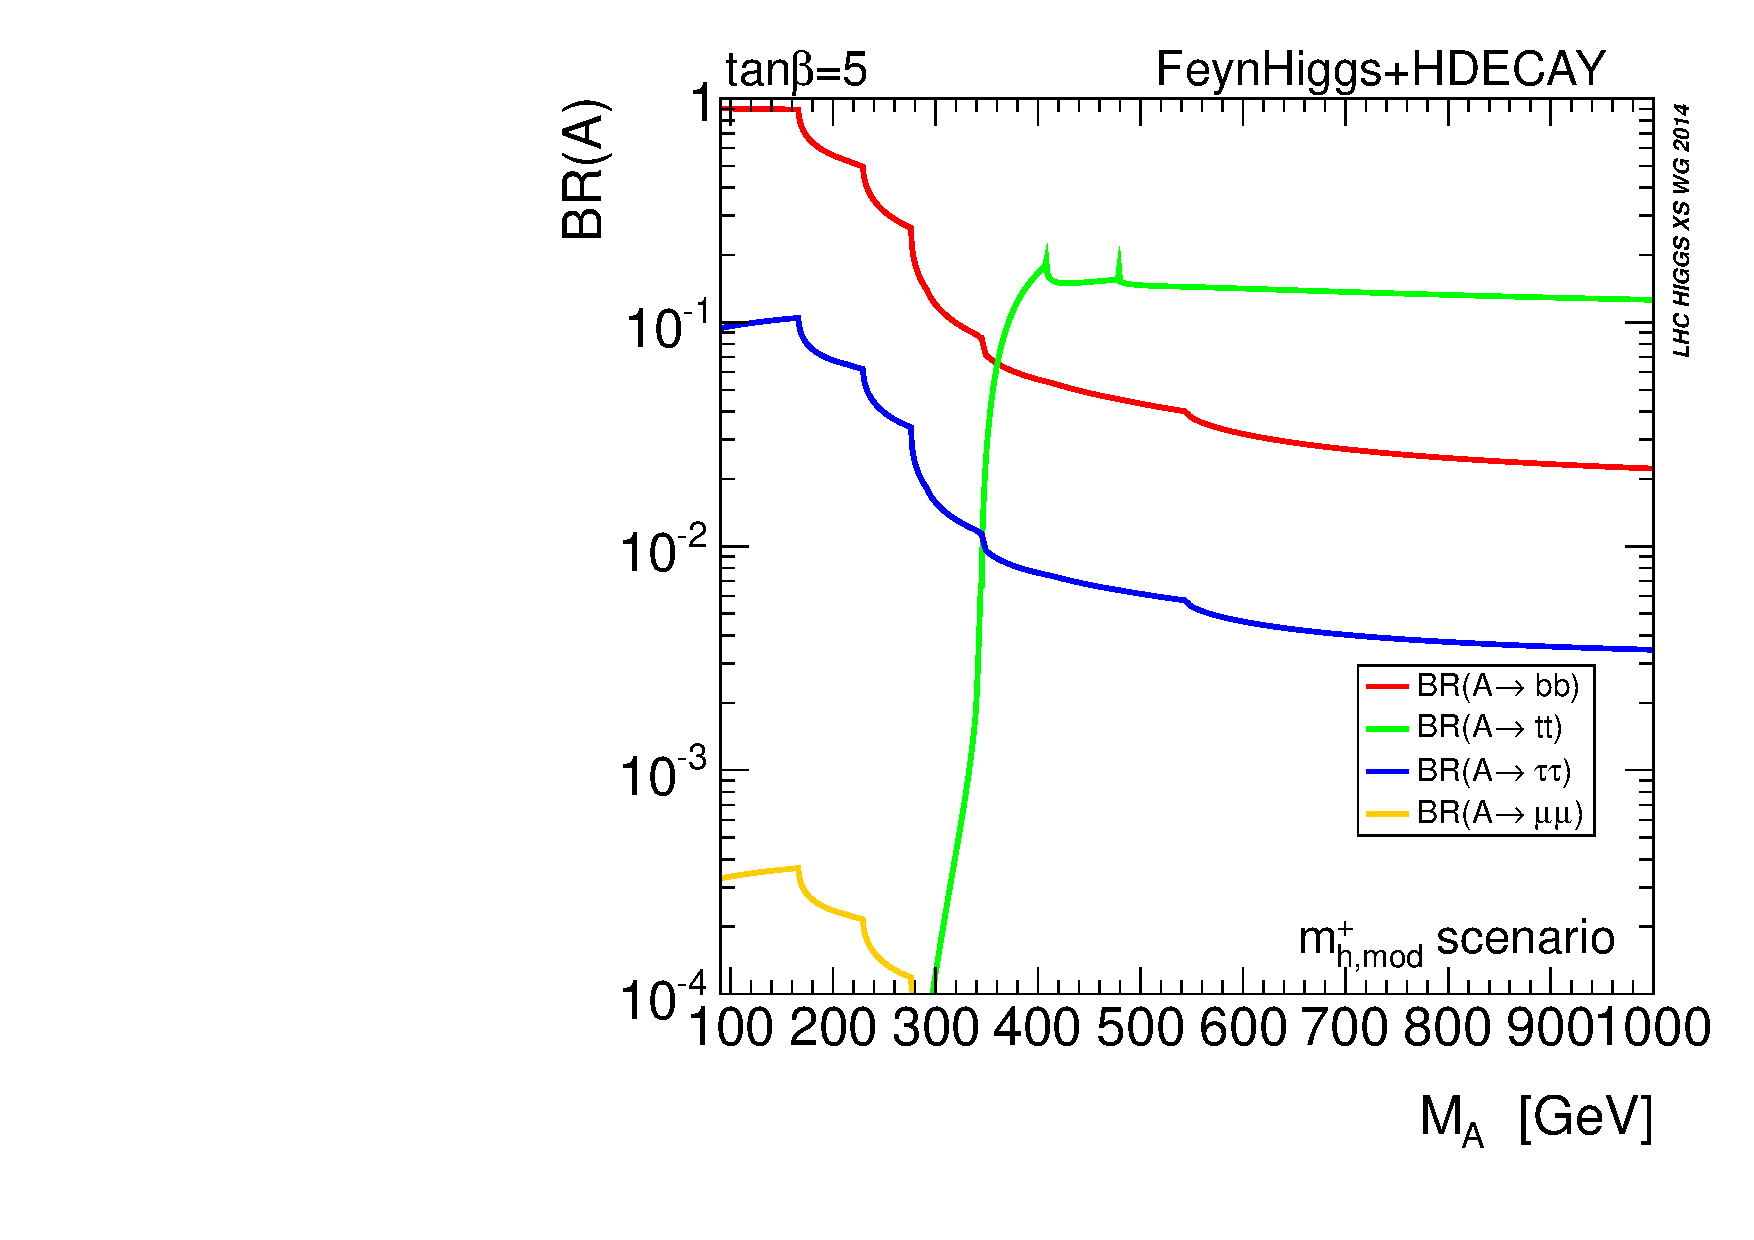
\includegraphics[width=0.49\columnwidth]{figures_chapter2/YR4HXS_BRSummary_A_mhmodp_tanbeta5_FeynHiggs_HDecay}
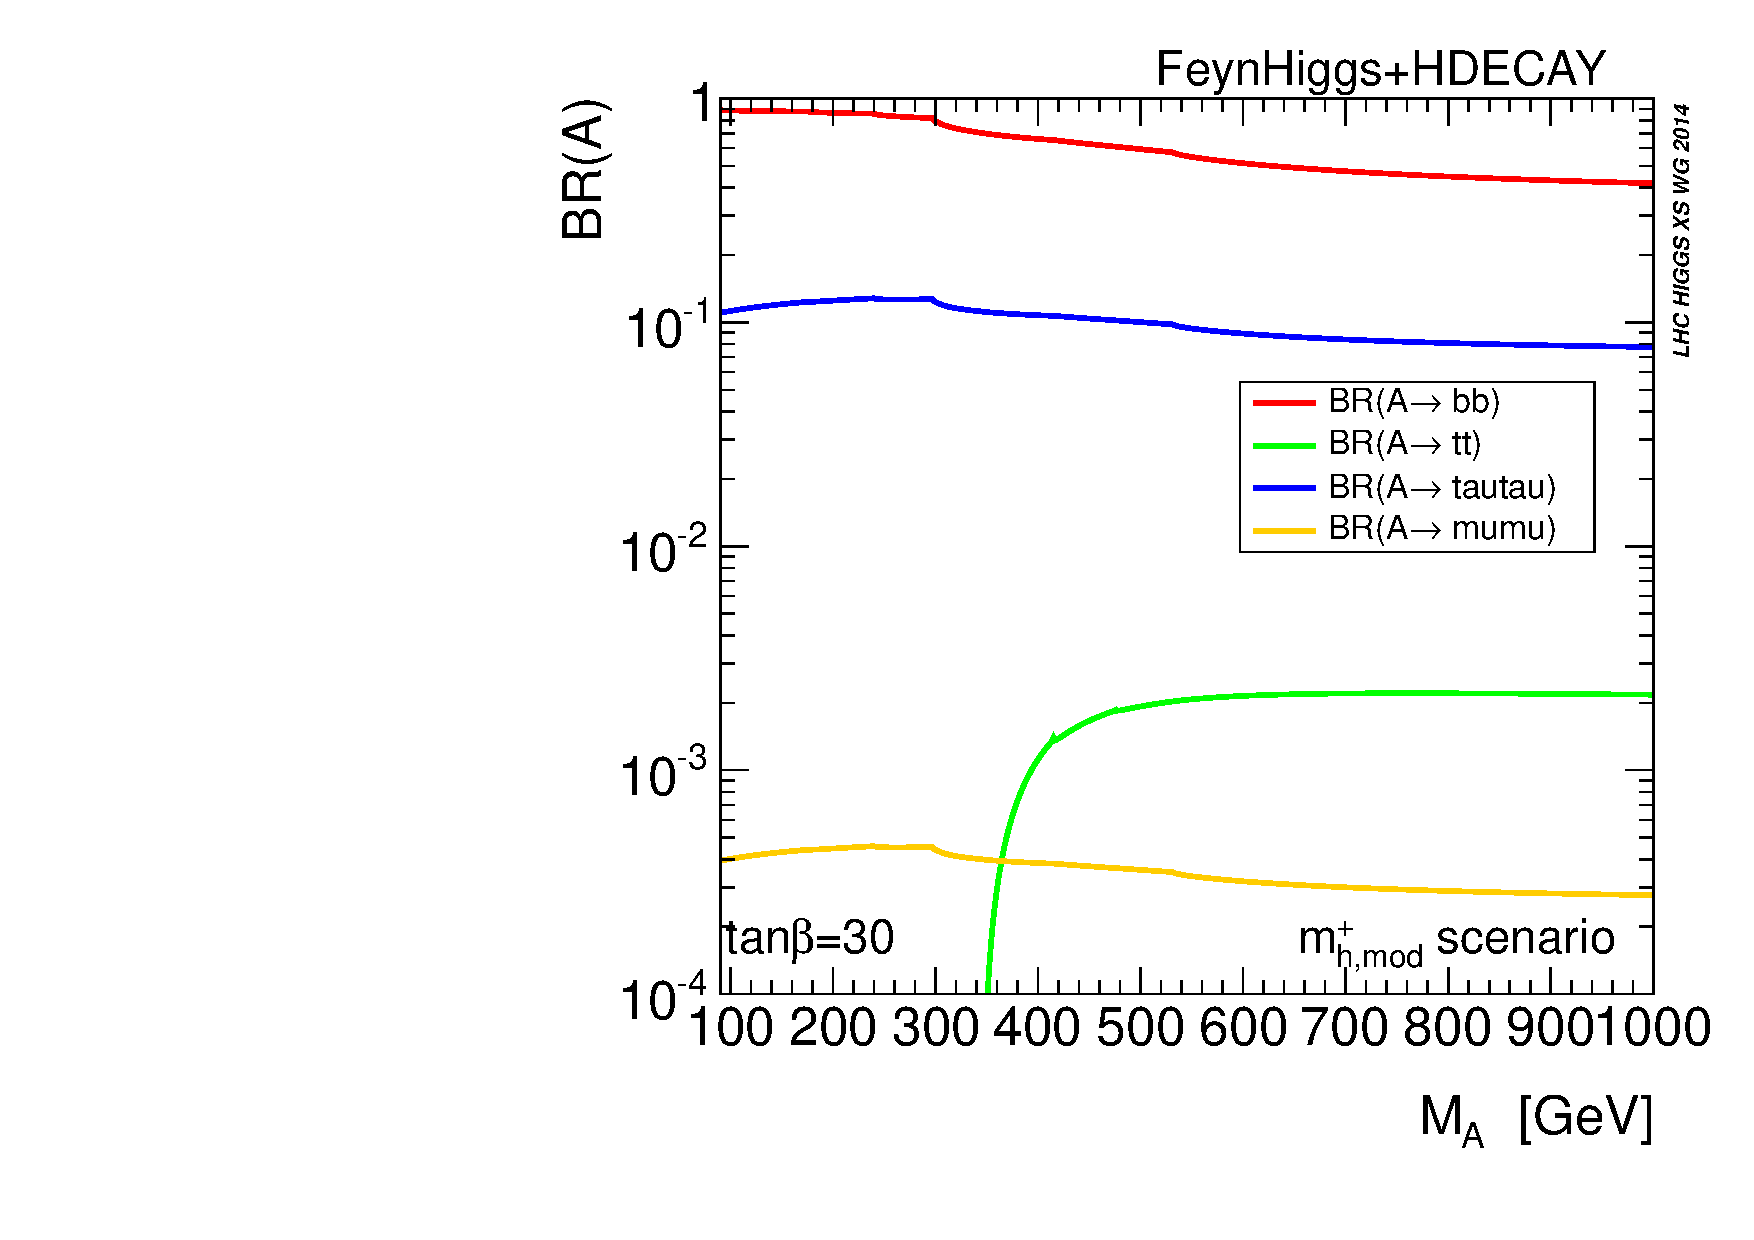
\includegraphics[width=0.49\columnwidth]{figures_chapter2/YR4HXS_BRSummary_A_mhmodp_tanbeta30_FeynHiggs_HDecay}
\caption{Neutral CP-odd Higgs boson branching fractions as a function of the mass in the $m_{h}^{mod+}$ benchmark scenario with $\tan \beta = 5$ (left panel) and $\tan \beta = 30$ (right panel)~\cite{Dittmaier:2011ti,Dittmaier:2012vm,Heinemeyer:2013tqa}} 
\label{fig:mssm_decay}
\end{figure} 

The main MSSM Higgs boson production modes are shown in Figure~\ref{fig:mssm_feynman}. The gluon fusion and associated b quark production modes dominate. The production cross sections of the three neutral Higgs bosons $h$, $H$, and $A$ for one of the commonly used benchmark scenarios are shown in Figure~\ref{fig:mssm_cross} at $\sqrt{s}=8~\TeV$ as a function of the CP-odd Higgs mass. The left (right) panel shows the cross sections with $\tan \beta = 5$ ($\tan \beta =30$).  The b quark associated production cross section is enhanced for larger $\tan \beta$ values as the coupling of the neutral MSSM Higgs bosons to fermions scales with $\tan \beta$. Correspondingly the heavy neutral bosons $H$ and $A$ mainly decay to $b\bar{b}$ and $\tau\tau$ final states for large values of $\tan \beta$. Figure~\ref{fig:mssm_decay} shows the branching fractions of the CP-odd Higgs as a function of the mass with $\tan \beta=5$ (left) and $\tan \beta=30$ (right). Thus, the search for the MSSM heavy neutral Higgs bosons with $\tau\tau$ decay channel is strongly motivated taking into account the experimental difficulties of the searches with the $b\bar{b}$ decay channel.
   